\documentclass[12pt]{article}

\usepackage{preamble}

%! Author = sbbfti
%! Date = 10/06/2020

\newacronym{ADF}{ADF test}{Augmented Dickey-Fuller test}
\newacronym{KPSS}{KPSS test}{Kwiatkowski-Phillips-Schmidt-Shin test}
\newacronym{ACF}{ACF}{AutoCorrelation function}
\newacronym{PACF}{PACF}{Partial AutoCorrelation function}


\newacronym{ti}{$T_{i}$}{indoor air temperature, $^{\circ}$C}



\begin{document}

%%%%%%%%%%%%%%%%%%%%%%%%%%%%%%%%%%%%%%%%%%%%%%%%%%%%%%%%%%%%%%%%%


\begin{titlepage}
	\centering
    \vspace*{0.4 cm}
    
\includegraphics[scale = 0.5]{figures/unb.jpg}\\[1.0 cm]	% University Logo
    \textsc{\LARGE \newline\newline University of New Brunswick}\\[1.8 cm]	% University Name
	\textsc{\Large Time Series Analysis\\(EE 6563)}\\[0.5 cm]				% Course Code
	\rule{\linewidth}{0.2 mm} \\[0.4 cm]
	{ \huge \bfseries \thetitle}\\
	\rule{\linewidth}{0.2 mm} \\[1.5 cm]
	
	\begin{minipage}{0.5\textwidth}
		\begin{flushleft} \large
			\emph{Professor:}\\
			Erik Scheme\\
            Electrical and Computer Engineering\\
			\end{flushleft}
			\end{minipage}~
			\begin{minipage}{0.5\textwidth}
            
			\begin{flushright} \large
			\emph{Author:} \\
			Saeed Kazemi\\ (3713280)\\

		\end{flushright}
        
	\end{minipage}\\[1 cm]
	
	
    \thedate
    
    
    
	
\end{titlepage}

%%%%%%%%%%%%%%%%%%%%%%%%%%%%%%%%%%%%%%%%%%%%%%%%%%%%%%%%%%%%%%%%%



%\tableofcontents
\pagebreak

%%%%%%%%%%%%%%%%%%%%%%%%%%%%%%%%%%%%%%%%%%%%%%%%%%%%%%%%%%%%%%%%%
%================================================================
\begin{enumerate}


%%%%%%%%%%%%%%%%%%%%%%%%%%%%%%%%%%%%%%%%%%%%%%%%%%%%%%%%%%%%%%%%%
%%%%%%%%%%%%%%%%%%%%%%%% Question 1 %%%%%%%%%%%%%%%%%%%%%%%%%%%%%
%%%%%%%%%%%%%%%%%%%%%%%%%%%%%%%%%%%%%%%%%%%%%%%%%%%%%%%%%%%%%%%%%
\item \textbf{For each dataset, visualize the raw signals, identify any trends, seasonality, and/or other components, and try to remove them. Remember that you are not limited to the tools shown in the tutorial and should explore the various concepts discussed in class. You do not need to explain the theory behind the approaches, but you should provide justification for their use, and discussion of their results.}


\textit{Figures \ref{fig:Ass1_D1_raw_signal} and \ref{fig:Ass1_D2_raw_signal} indicate the raw signal of both data sets. Likewise, figure \ref{fig:Ass1_D1_raw_signal_1986} to  \ref{fig:Ass1_D2_raw_signal_1990} illustrate a short period in two datasets. }

\begin{figure}[H]
    \centering
    \begin{minipage}[b]{1\textwidth}
        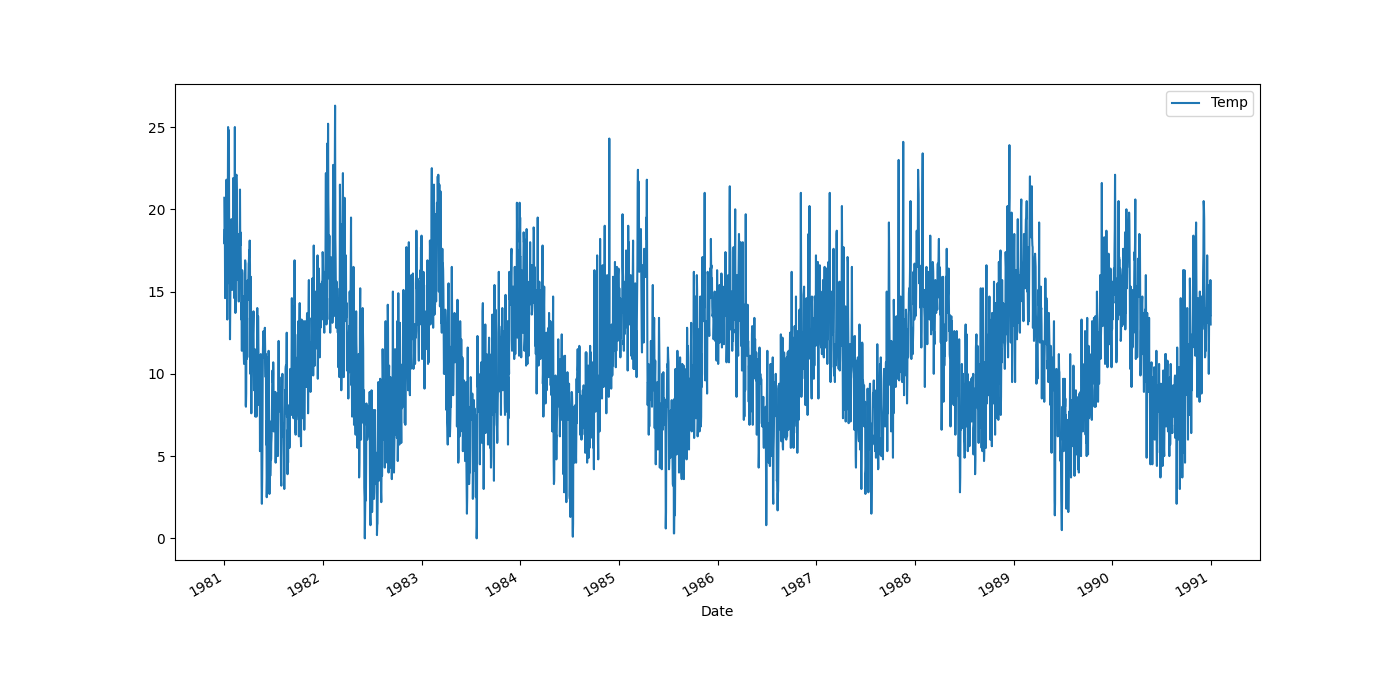
\includegraphics[width=\textwidth]{figures/Ass1/Ass1_D1_raw_signal.png}
    \end{minipage}
    \caption{The raw signal of the first dataset.}
    \label{fig:Ass1_D1_raw_signal}
\end{figure}

\begin{figure}[H]
    \centering
    \begin{minipage}[b]{1\textwidth}
        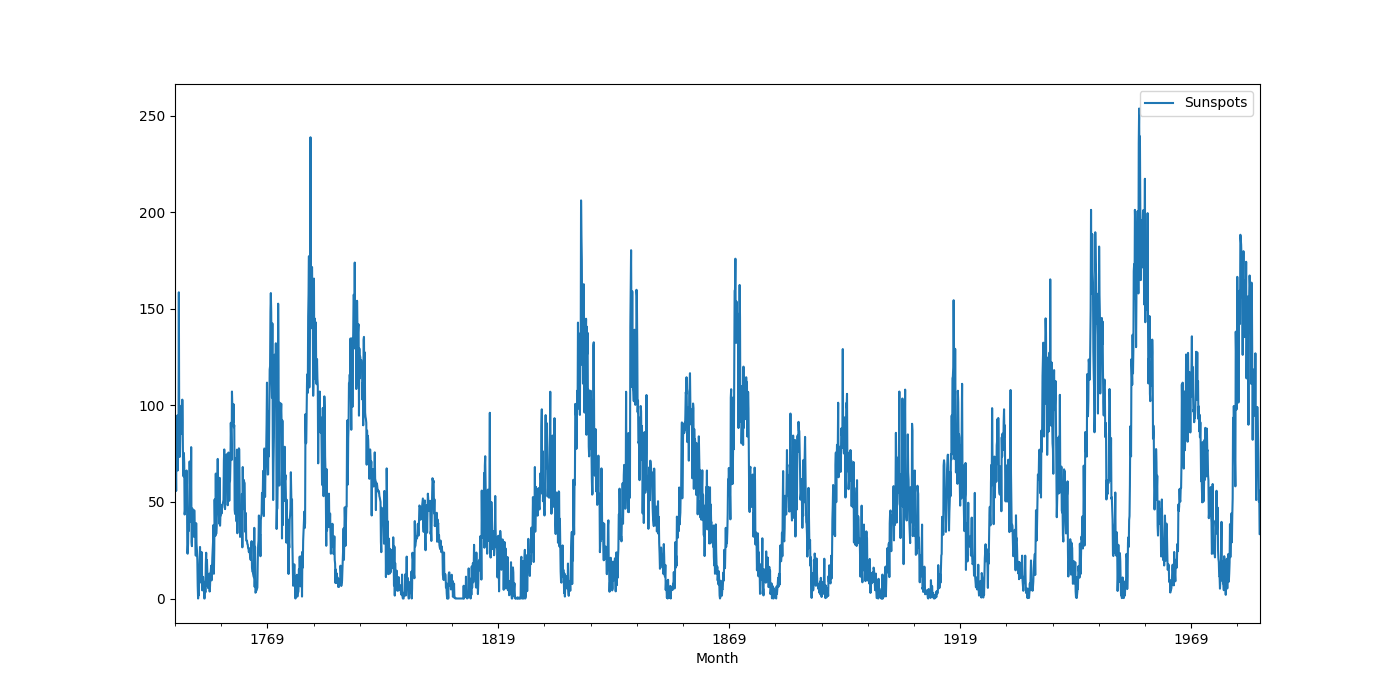
\includegraphics[width=\textwidth]{figures/Ass1/Ass1_D2_raw_signal.png}
    \end{minipage}
    \caption{The raw signal of the second dataset.}
    \label{fig:Ass1_D2_raw_signal}
\end{figure}

\begin{figure}[H]
    \centering
    \begin{minipage}[b]{1\textwidth}
        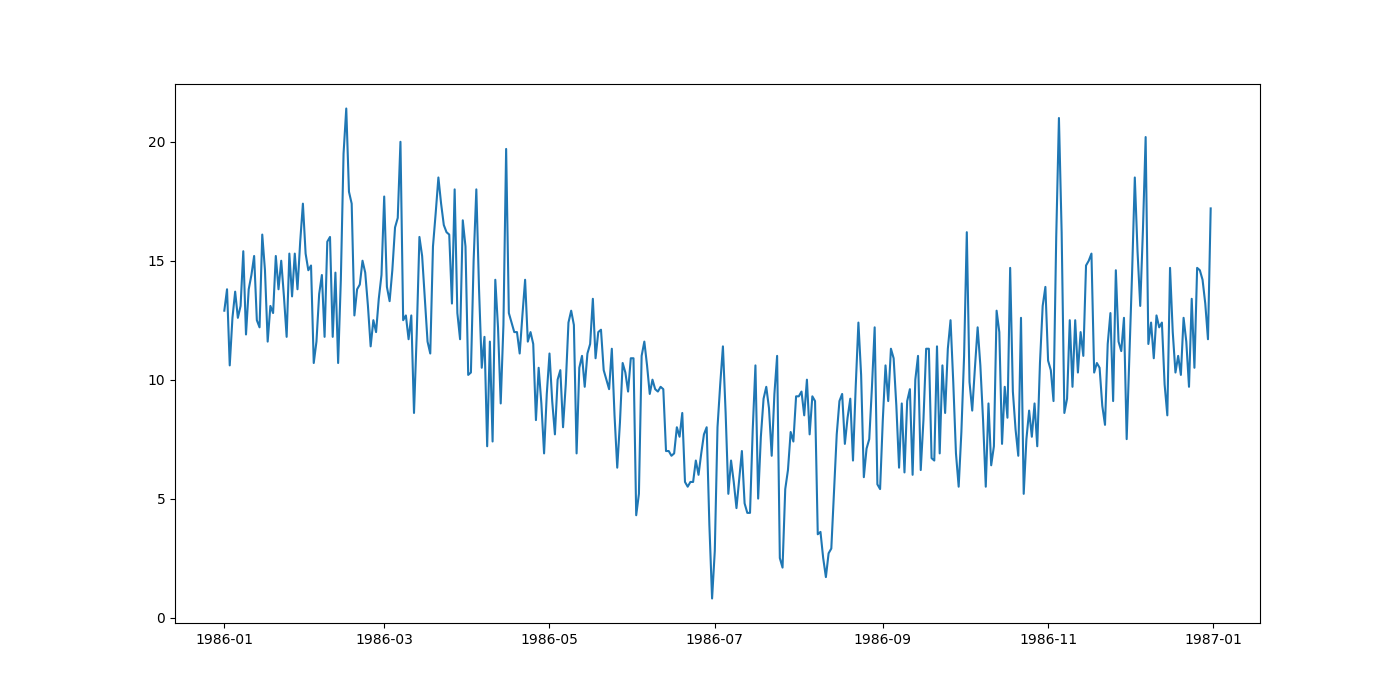
\includegraphics[width=\textwidth]{figures/Ass1/Ass1_D1_raw_signal_1986.png}
    \end{minipage}
    \caption{Visualizing a short period of the first dataset.}
    \label{fig:Ass1_D1_raw_signal_1986}
\end{figure}


\begin{figure}[H]
    \centering
    \begin{minipage}[b]{1\textwidth}
        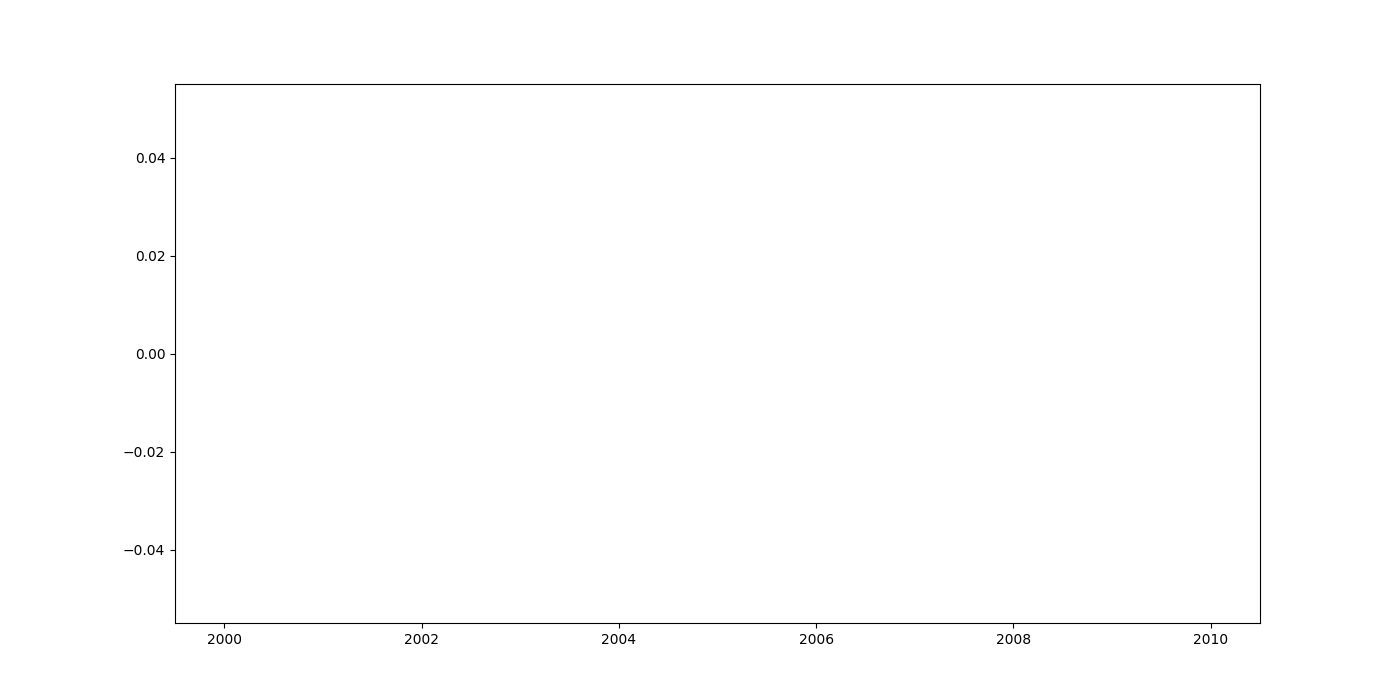
\includegraphics[width=\textwidth]{figures/Ass1/Ass1_D2_raw_signal_1990.png}
    \end{minipage}
    \caption{Visualizing a short period of the second dataset.}
    \label{fig:Ass1_D2_raw_signal_1990}
\end{figure}

\textit{For intuition, Table \ref{tab:Ass1_D1_raw_signal} to  \ref{tab:Ass1_D2_raw_signal_summary_statistics} show the top raw of two datasets along with the descriptive statistics of two time-series datasets.}


\begin{table}[H]
 \centering
\caption{The first five rows of the raw signal in the first dataset.}
\label{tab:Ass1_D1_raw_signal}
\begin{tabular}{lr}
\toprule
{} &  Temp \\
Date       &       \\
\midrule
1981-01-01 &  20.7 \\
1981-01-02 &  17.9 \\
1981-01-03 &  18.8 \\
1981-01-04 &  14.6 \\
1981-01-05 &  15.8 \\
1981-01-06 &  15.8 \\
1981-01-07 &  15.8 \\
\bottomrule
\end{tabular}

\end{table}

\begin{table}[H]
 \centering
\caption{The descriptive statistics of the first dataset.}
\label{tab:Ass1_D1_raw_signal_summary_statistics}
\begin{tabular}{lr}
\toprule
{} &         Temp \\
\midrule
count &  3650.000000 \\
mean  &    11.177753 \\
std   &     4.071837 \\
min   &     0.000000 \\
25\%   &     8.300000 \\
50\%   &    11.000000 \\
75\%   &    14.000000 \\
max   &    26.300000 \\
\bottomrule
\end{tabular}

\end{table}

\begin{table}[H]
 \centering
\caption{The first five rows of the raw signal in the second dataset.}
\label{tab:Ass1_D2_raw_signal}
\begin{tabular}{lr}
\toprule
{} &  Sunspots \\
Month      &           \\
\midrule
1749-01-01 &      58.0 \\
1749-02-01 &      62.6 \\
1749-03-01 &      70.0 \\
1749-04-01 &      55.7 \\
1749-05-01 &      85.0 \\
\bottomrule
\end{tabular}

\end{table}

\begin{table}[H]
 \centering
\caption{The descriptive statistics of the second dataset.} \label{tab:Ass1_D2_raw_signal_summary_statistics}
\begin{tabular}{lr}
\toprule
{} &     Sunspots \\
\midrule
count &  2820.000000 \\
mean  &    51.265957 \\
std   &    43.448971 \\
min   &     0.000000 \\
25\%   &    15.700000 \\
50\%   &    42.000000 \\
75\%   &    74.925000 \\
max   &   253.800000 \\
\bottomrule
\end{tabular}

\end{table}






\textit{For decomposing the time series, the below methods used:}
    \begin{enumerate}
    \item \textit{Seasonal\_decompose (Figure
        \ref{fig:Ass1_D1_seasonal_decompose} and \ref{fig:Ass1_D2_seasonal_decompose})}
        
    \item \textit{STL (Figure
        \ref{fig:Ass1_D1_STL} and \ref{fig:Ass1_D2_STL})}
        
    \item \textit{Linear Regression method (Figure
        \ref{fig:Ass1_D1_LinearRegression_diff} and \ref{fig:Ass1_D2_LinearRegression_diff})}
        
    \item \textit{Difference method (Figure
        \ref{fig:Ass1_D1_one_diff} and \ref{fig:Ass1_D2_one_diff})}
        
    \item \textit{Fitting a polynomial (Figure
        \ref{fig:Ass1_D1_fiting_polynomial} and \ref{fig:Ass1_D2_fiting_polynomial})}
        
    \item \textit{Moving Average window (Figure
        \ref{fig:Ass1_D1_Moving_Avrage} and \ref{fig:Ass1_D2_Moving_Avrage})}

    \end{enumerate}

\textit{\newline \newline Some mentioned methods used only for extracting only one type of component (trend or seasonality), while others like STL 
and Seasonal\_decompose provided all three parts. Table \ref{tab:Ass1_comparing_methods} compares these methods together.}

\textit{Also, there are two models for the reconstruction of time series, Additive and Multiplicative Model. In this assignment, the additive model was only used because the multiplicative model is not appropriate for zero and negative values.}

\begin{table}[H]
\centering
\caption{Comparing the implemented methods.}
\label{tab:Ass1_comparing_methods}
\begin{tabular}{@{}lccc@{}}
\toprule
                    & \begin{tabular}[c]{@{}c@{}}Trend \\ component\end{tabular} & \begin{tabular}[c]{@{}c@{}}Seasonal \\ component\end{tabular} & \begin{tabular}[c]{@{}c@{}}Residual \\ component\end{tabular} \\ \midrule
Seasonal\_decompose & \checkmark                                  & \checkmark                                     & \checkmark                                     \\ \midrule
STL                 & \checkmark                                  & \checkmark                                     & \checkmark                                     \\ \midrule
Linear Regression   & \checkmark                                  & -                                                             & -                                                             \\ \midrule
Difference          & -                                                          & \checkmark                                     & -                                                             \\ \midrule
Moving average      & \checkmark                                  & -                                                             & -                                                             \\ \bottomrule
\end{tabular}

\end{table}


\textit{For finding the seasonal component, we need to find the period of the time series. For doing this, the resampling method was used to smooth the plots of two datasets. Figures \ref{fig:Ass1_D1_resample} and \ref{fig:Ass1_D2_resample} indicate the smooth version of the two datasets. }

\begin{figure}[H]
    \centering
    \begin{minipage}[b]{1\textwidth}
        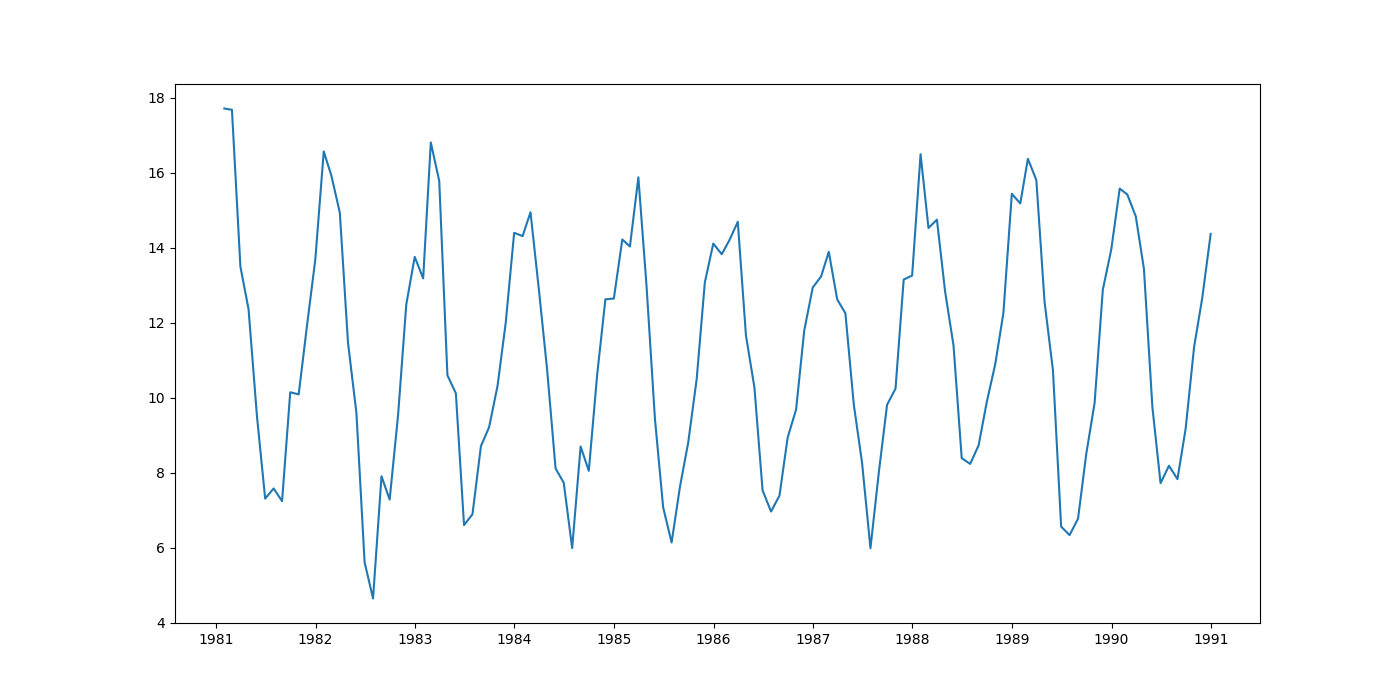
\includegraphics[width=\textwidth]{figures/Ass1/Ass1_D1_resample.png}
    \end{minipage}
    \caption{Resampling plot of the first dataset. The period of this dataset is 365 samples/cycle. }
    \label{fig:Ass1_D1_resample}
\end{figure}

\begin{figure}[H]
    \centering
    \begin{minipage}[b]{1\textwidth}
        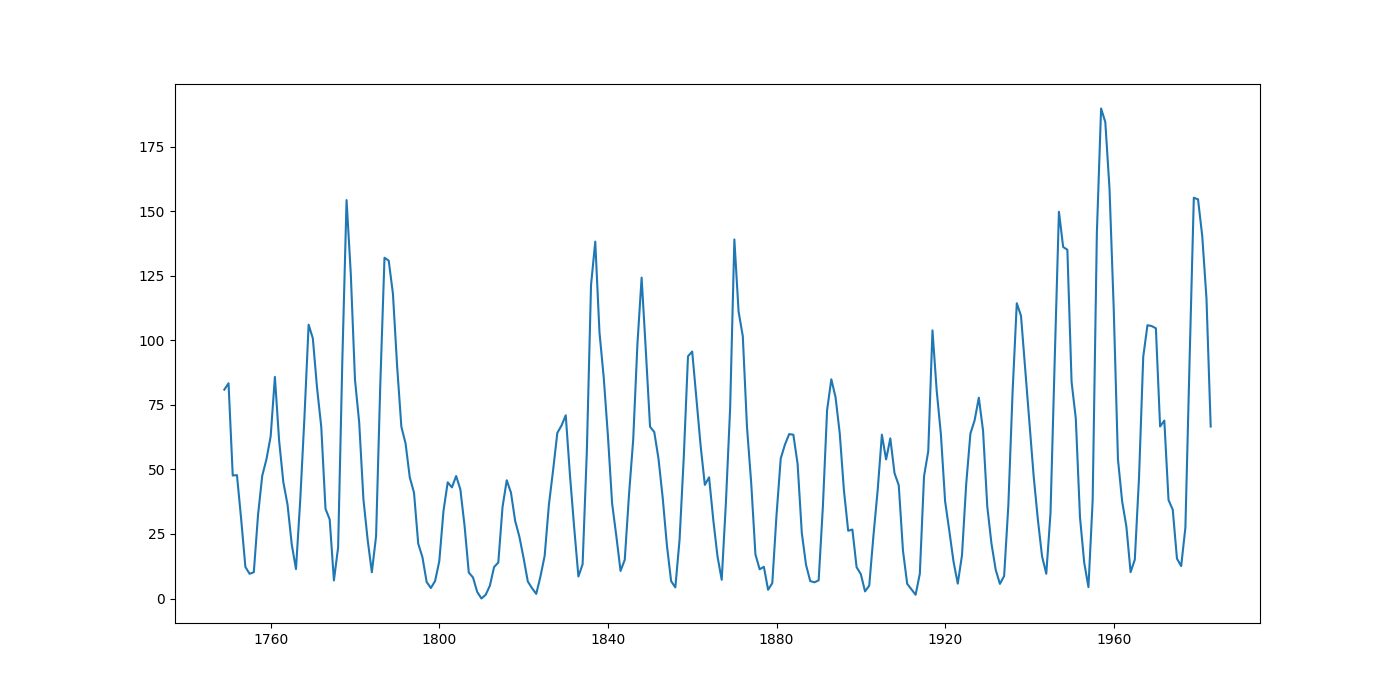
\includegraphics[width=\textwidth]{figures/Ass1/Ass1_D2_resample.png}
    \end{minipage}
    \caption{Resampling plot of the second dataset. The period of this dataset is 130 samples/cycle.}
    \label{fig:Ass1_D2_resample}
\end{figure}


\textit{Furthermore, the period of the time-series data can calculate by \gls{ACF} (figures \ref{fig:Ass1_D1_PACF_ACF_series} and \ref{fig:Ass1_D2_PACF_ACF_series}). This plot has an oscillation, indicative of a seasonal series and the peaks occurred at each period. }

\begin{figure}[H]
    \centering
    \begin{minipage}[b]{1\textwidth}
        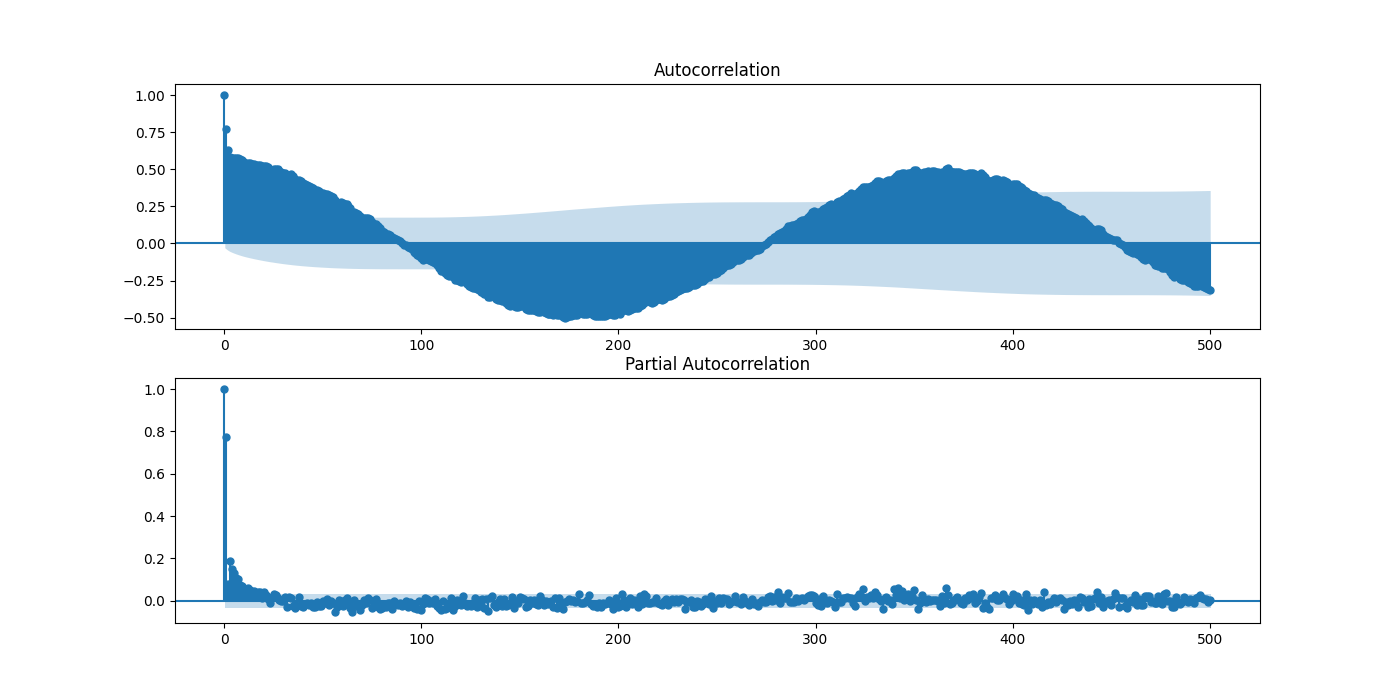
\includegraphics[width=\textwidth]{figures/Ass1/Ass1_D1_PACF_ACF_series.png}
    \end{minipage}
    \caption{The \gls{ACF} and \gls{PACF} of the first dataset. The peaks occur at the lag of 365 that means the period is 365 samples/cycle.}
    \label{fig:Ass1_D1_PACF_ACF_series}
\end{figure}

\begin{figure}[H]
    \centering
    \begin{minipage}[b]{1\textwidth}
        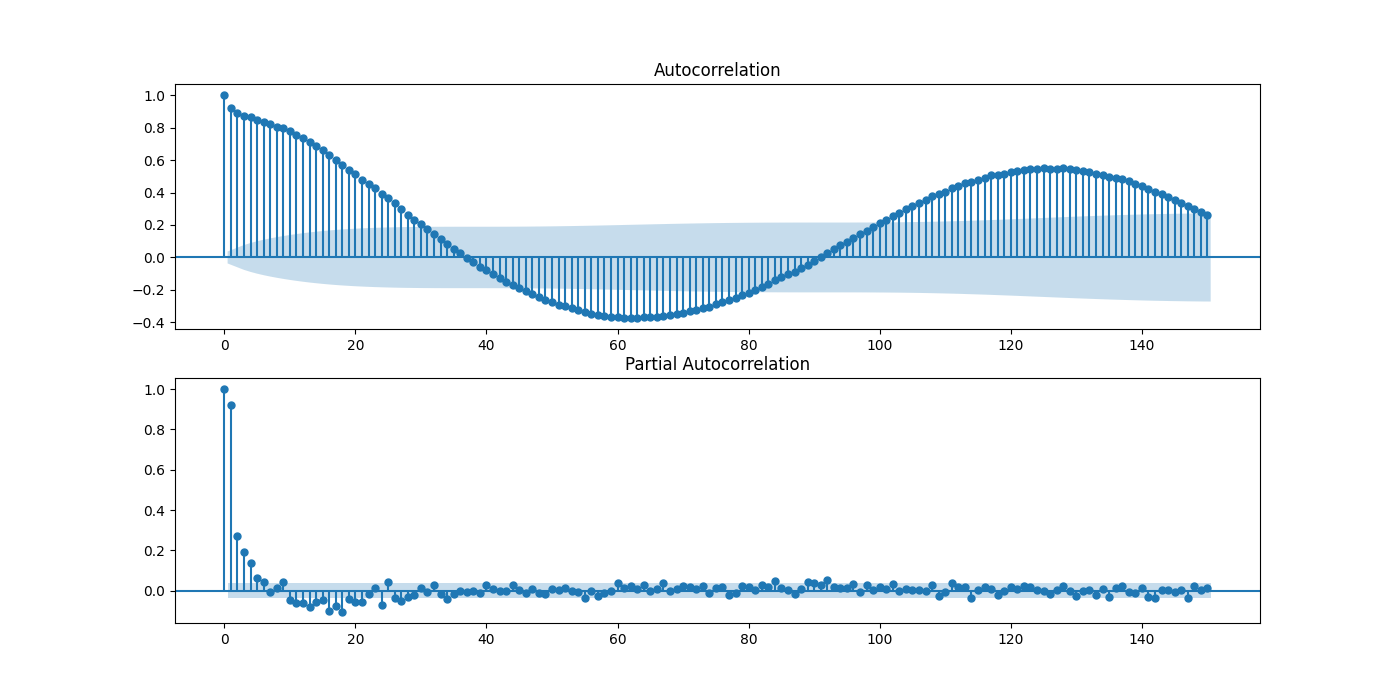
\includegraphics[width=\textwidth]{figures/Ass1/Ass1_D2_PACF_ACF_series.png}
    \end{minipage}
    \caption{The \gls{ACF} and \gls{PACF} of the second dataset. The peaks occur at the lag of 130 that means the period is 130 samples/cycle.}
    \label{fig:Ass1_D2_PACF_ACF_series}
\end{figure}


\begin{figure}[H]
    \centering
    \begin{minipage}[b]{1\textwidth}
        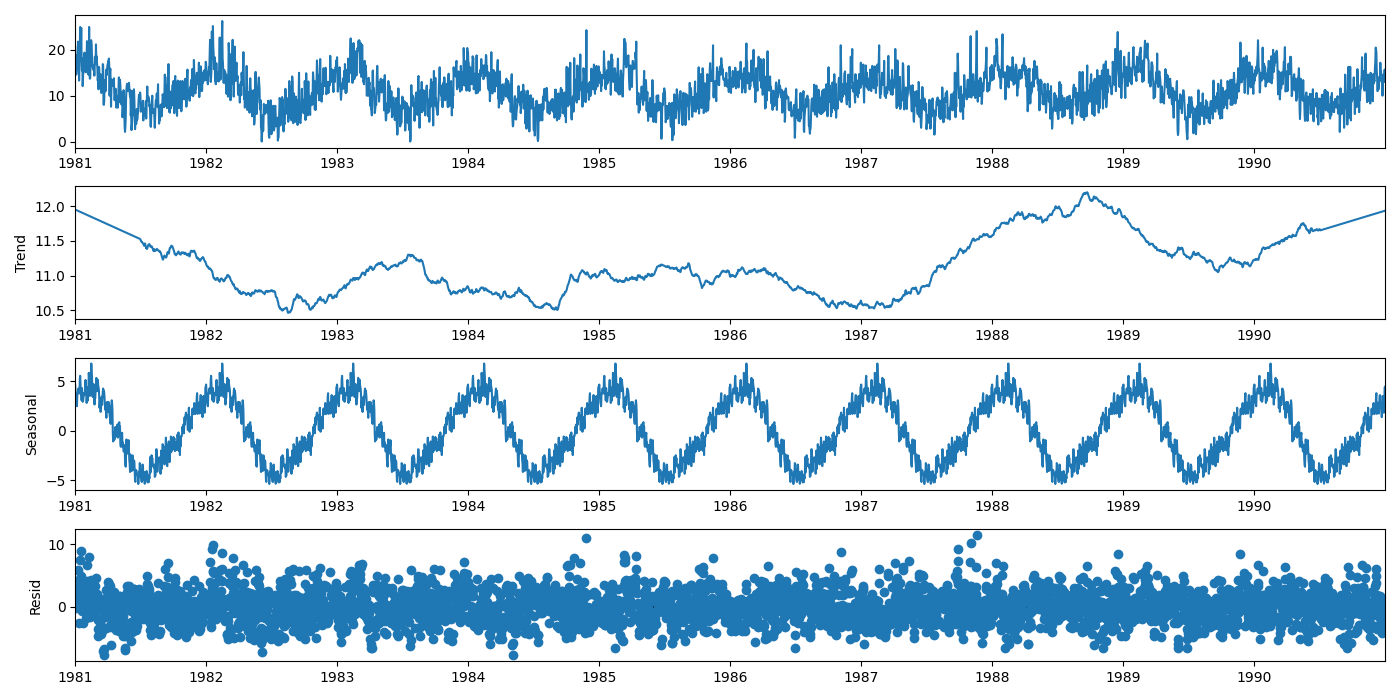
\includegraphics[width=\textwidth]{figures/Ass1/Ass1_D1_seasonal_decompose.png}
    \end{minipage}
    \caption{Decomposition of the first dataset by seasonal\_decompose method}
    \label{fig:Ass1_D1_seasonal_decompose}
\end{figure}

\begin{figure}[H]
    \centering
    \begin{minipage}[b]{1\textwidth}
        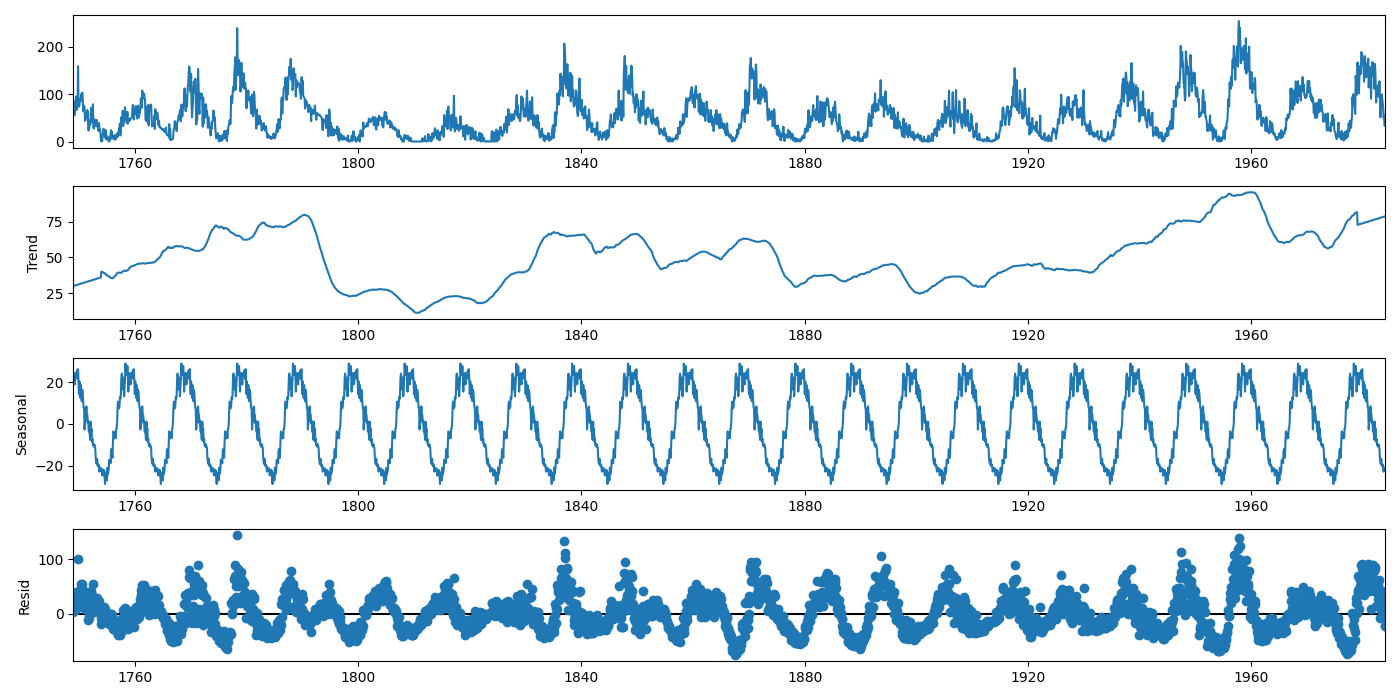
\includegraphics[width=\textwidth]{figures/Ass1/Ass1_D2_seasonal_decompose.png}
    \end{minipage}
    \caption{Decomposition of the second dataset by seasonal\_decompose method}
    \label{fig:Ass1_D2_seasonal_decompose}
\end{figure}

\begin{figure}[H]
    \centering
    \begin{minipage}[b]{1\textwidth}
        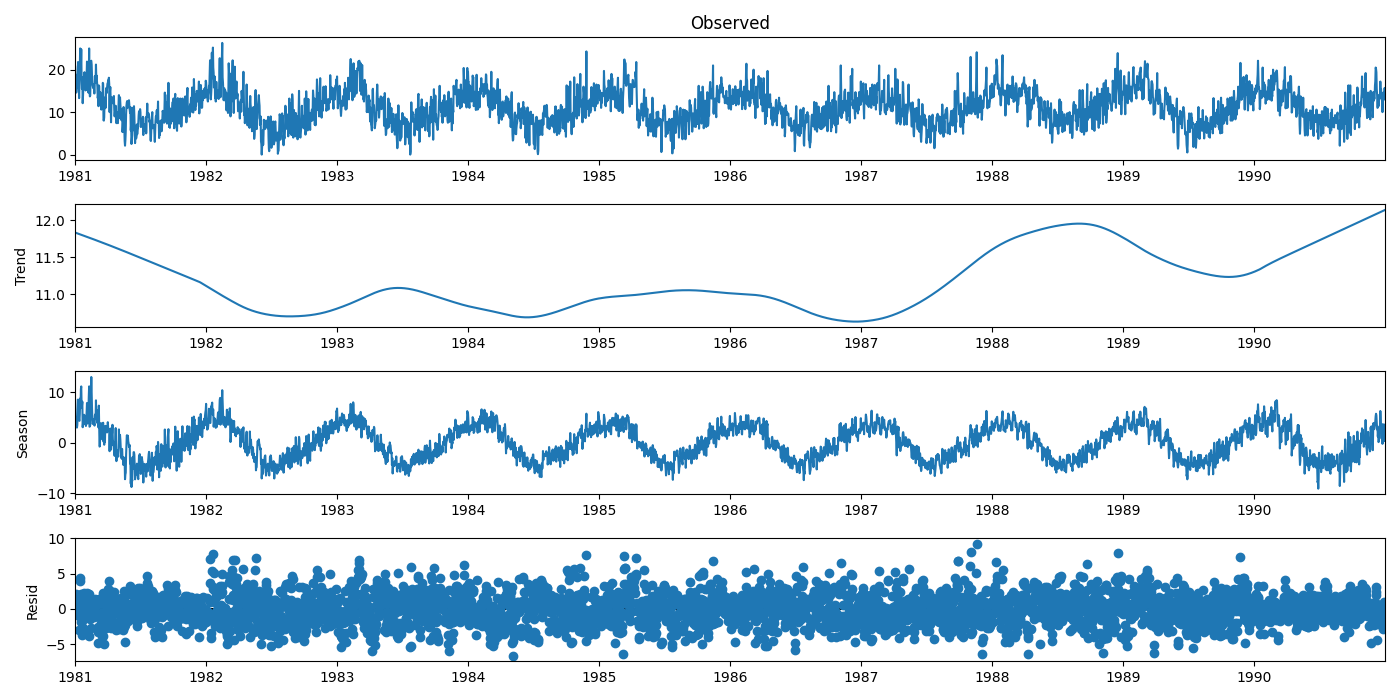
\includegraphics[width=\textwidth]{figures/Ass1/Ass1_D1_STL.png}
    \end{minipage}
    \caption{Decomposition of the first dataset by STL method}
    \label{fig:Ass1_D1_STL}
\end{figure}

\begin{figure}[H]
    \centering
    \begin{minipage}[b]{1\textwidth}
        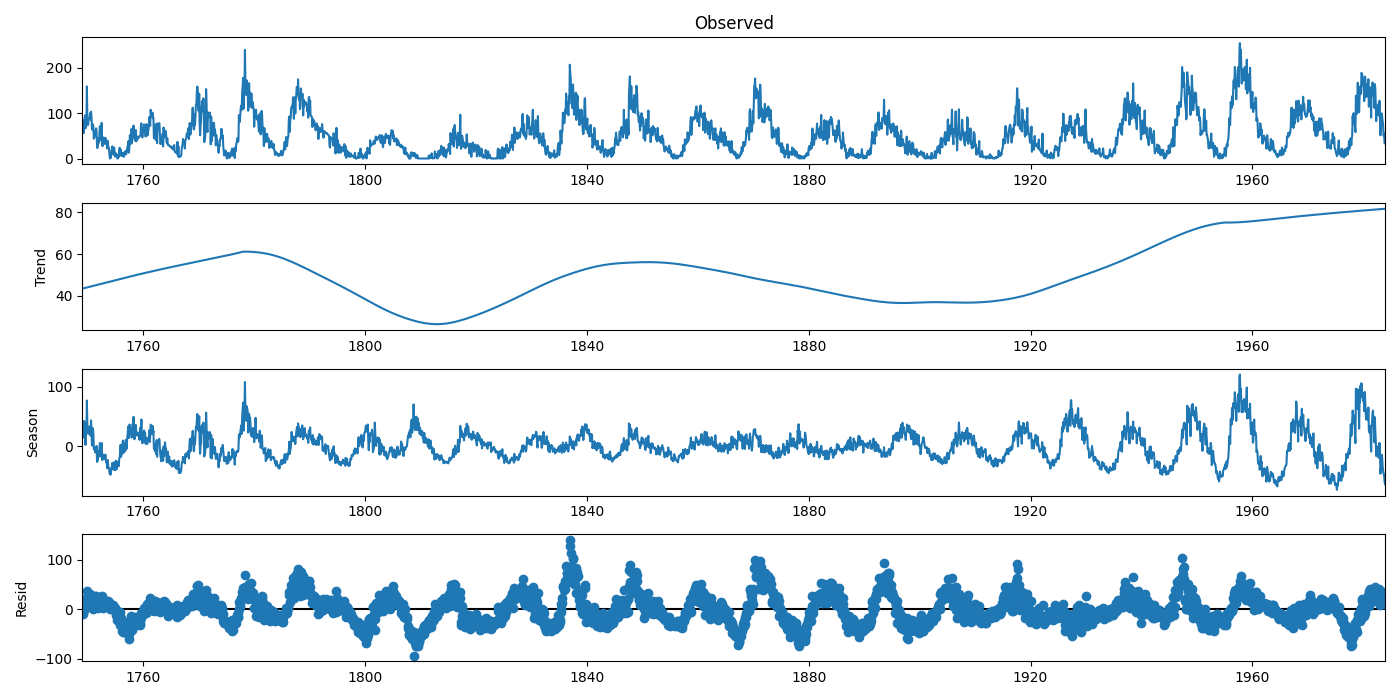
\includegraphics[width=\textwidth]{figures/Ass1/Ass1_D2_STL.png}
    \end{minipage}
    \caption{Decomposition of the second dataset by STL method}
    \label{fig:Ass1_D2_STL}
\end{figure}

\begin{figure}[H]
    \centering
    \begin{minipage}[b]{1\textwidth}
        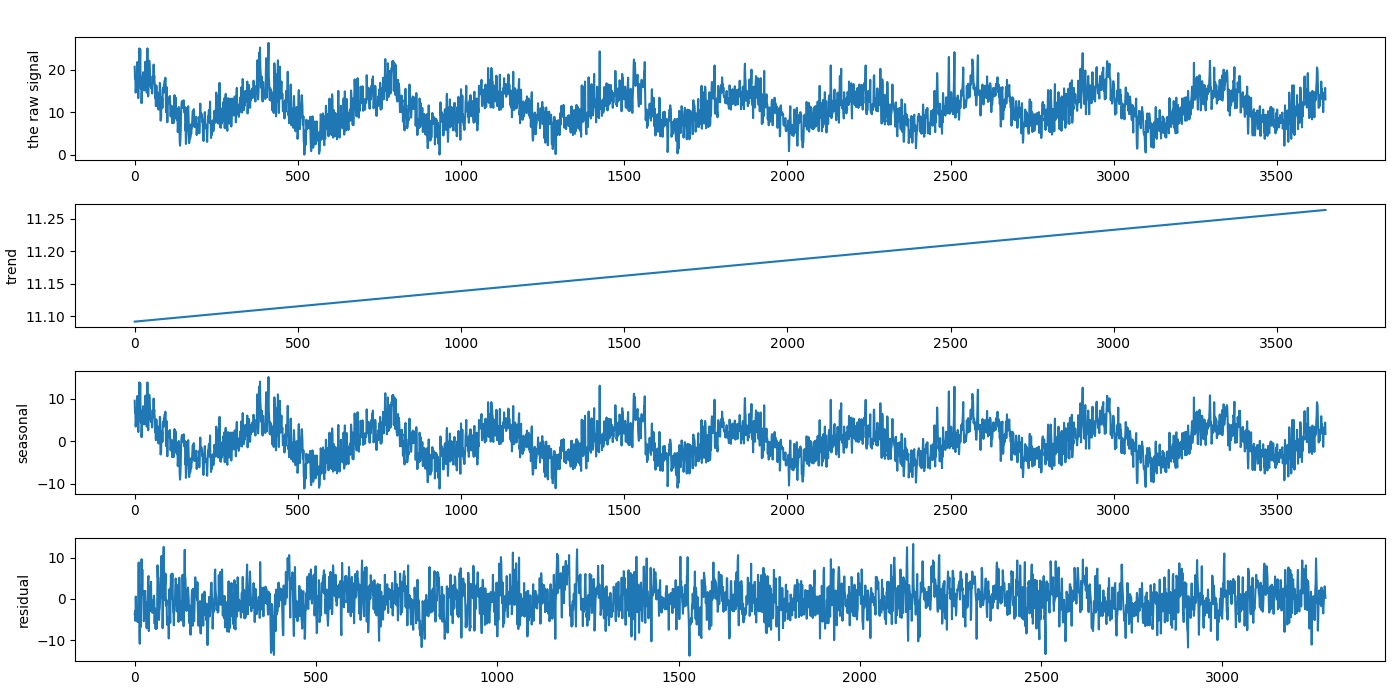
\includegraphics[width=\textwidth]{figures/Ass1/Ass1_D1_LinearRegression_diff.png}
    \end{minipage}
    \caption{Decomposition of the first dataset by Linear Regression and difference method.}
    \label{fig:Ass1_D1_LinearRegression_diff}
\end{figure}

\begin{figure}[H]
    \centering
    \begin{minipage}[b]{1\textwidth}
        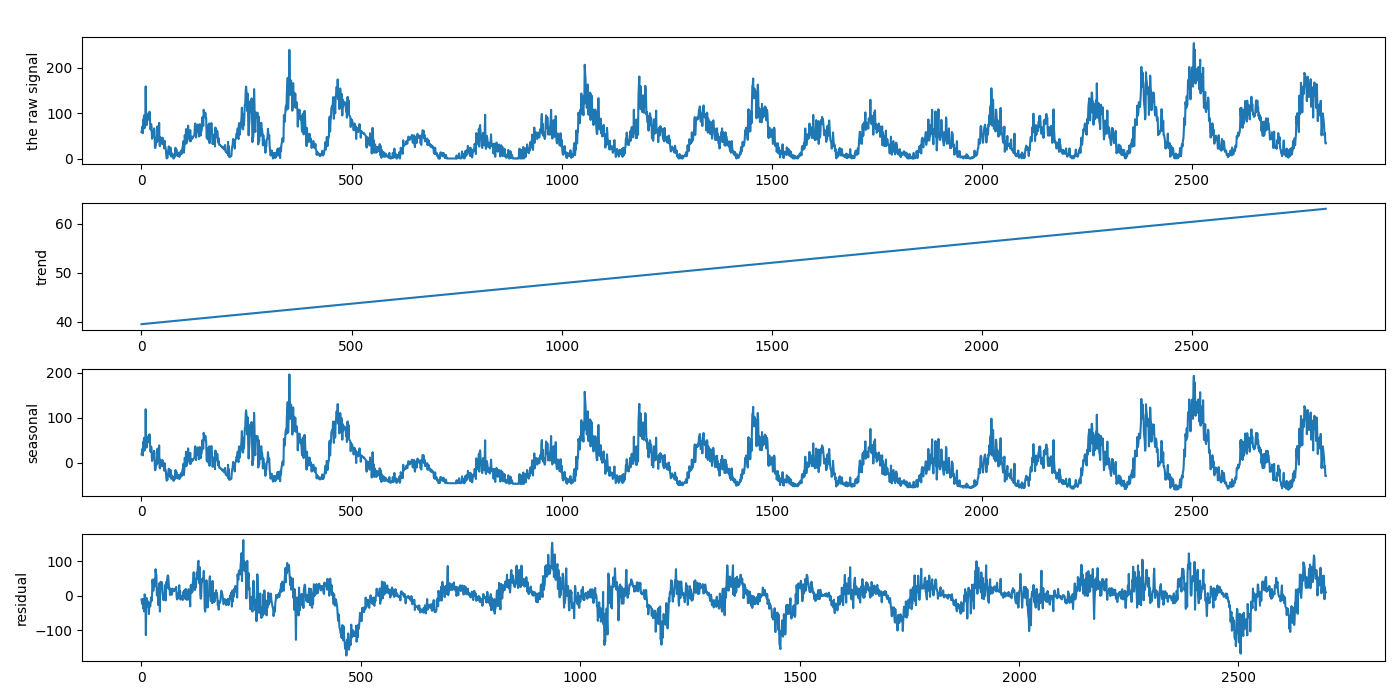
\includegraphics[width=\textwidth]{figures/Ass1/Ass1_D2_LinearRegression_diff.png}
    \end{minipage}
    \caption{Decomposition of the second dataset by Linear Regression and difference method.}
    \label{fig:Ass1_D2_LinearRegression_diff}
\end{figure}

\begin{figure}[H]
    \centering
    \begin{minipage}[b]{1\textwidth}
        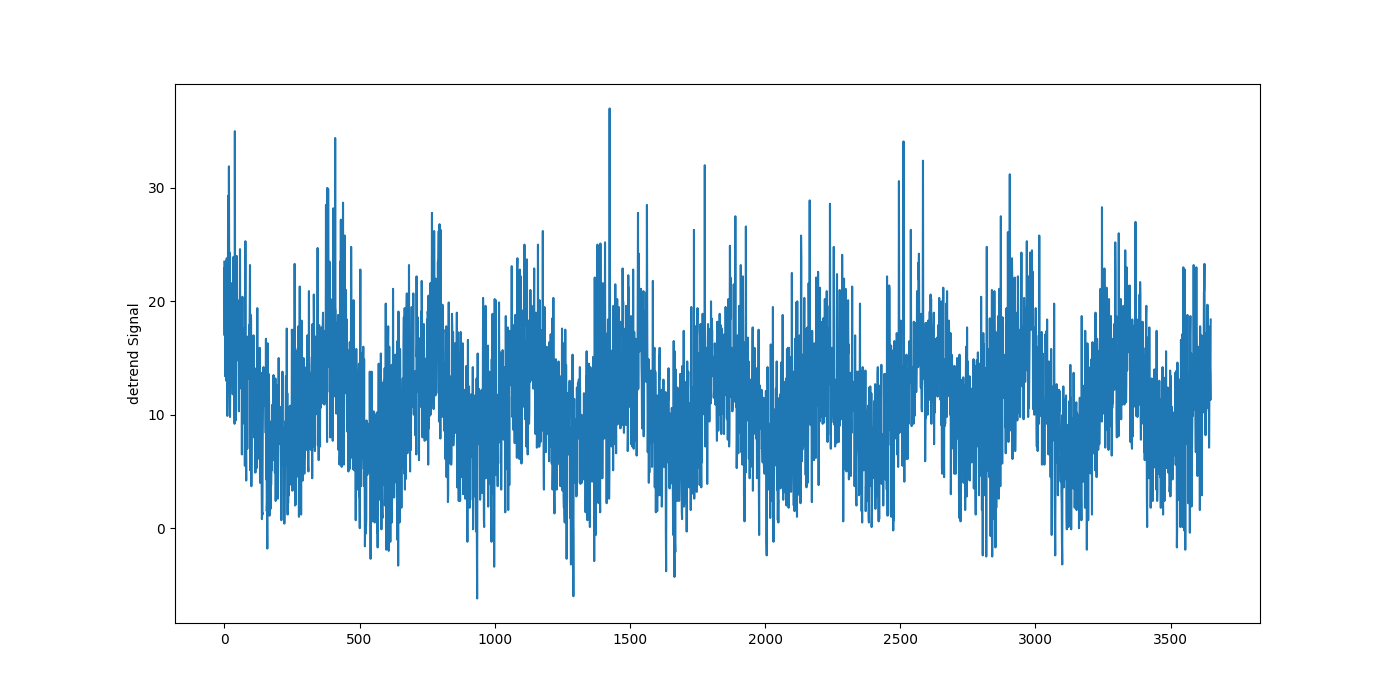
\includegraphics[width=\textwidth]{figures/Ass1/Ass1_D1_one_diff.png}
    \end{minipage}
    \caption{Detrending of the first dataset by the first-order differencing.}
    \label{fig:Ass1_D1_one_diff}
\end{figure}

\begin{figure}[H]
    \centering
    \begin{minipage}[b]{1\textwidth}
        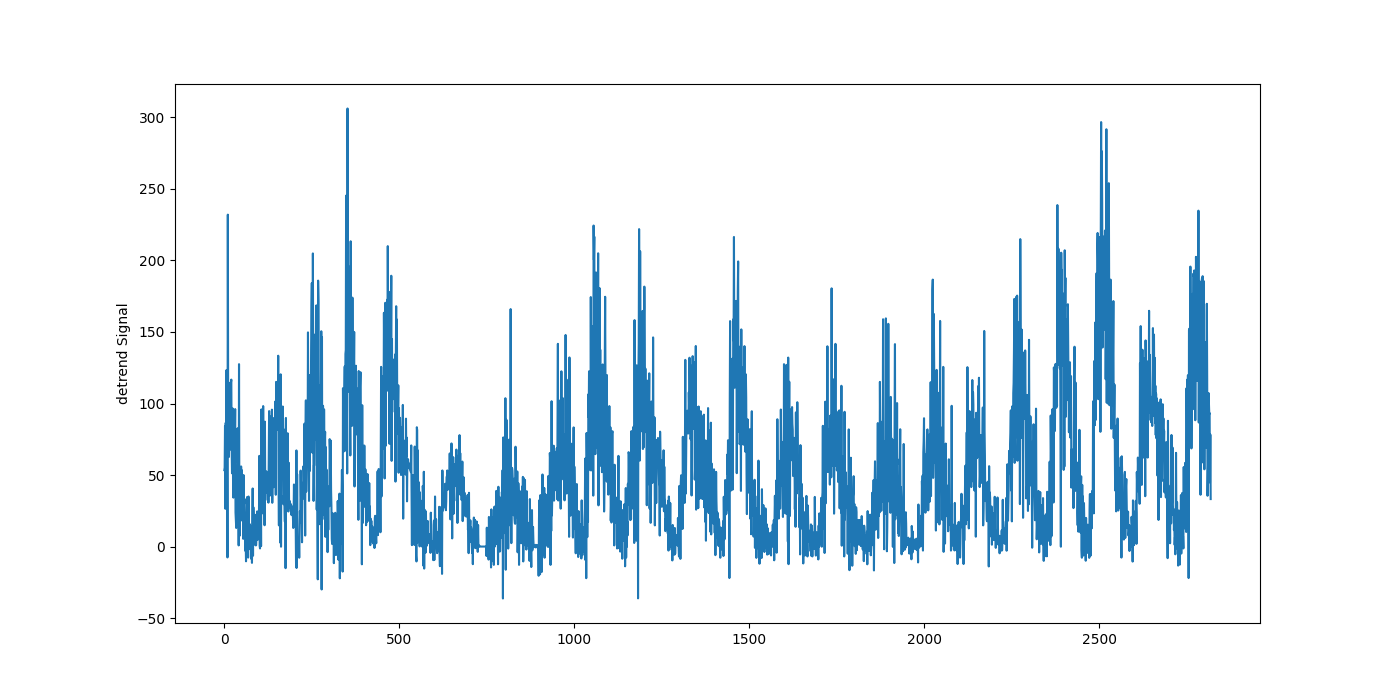
\includegraphics[width=\textwidth]{figures/Ass1/Ass1_D2_one_diff.png}
    \end{minipage}
    \caption{Detrending of the second dataset by the first-order differencing.}
    \label{fig:Ass1_D2_one_diff}
\end{figure}

\begin{figure}[H]
    \centering
    \begin{minipage}[b]{1\textwidth}
        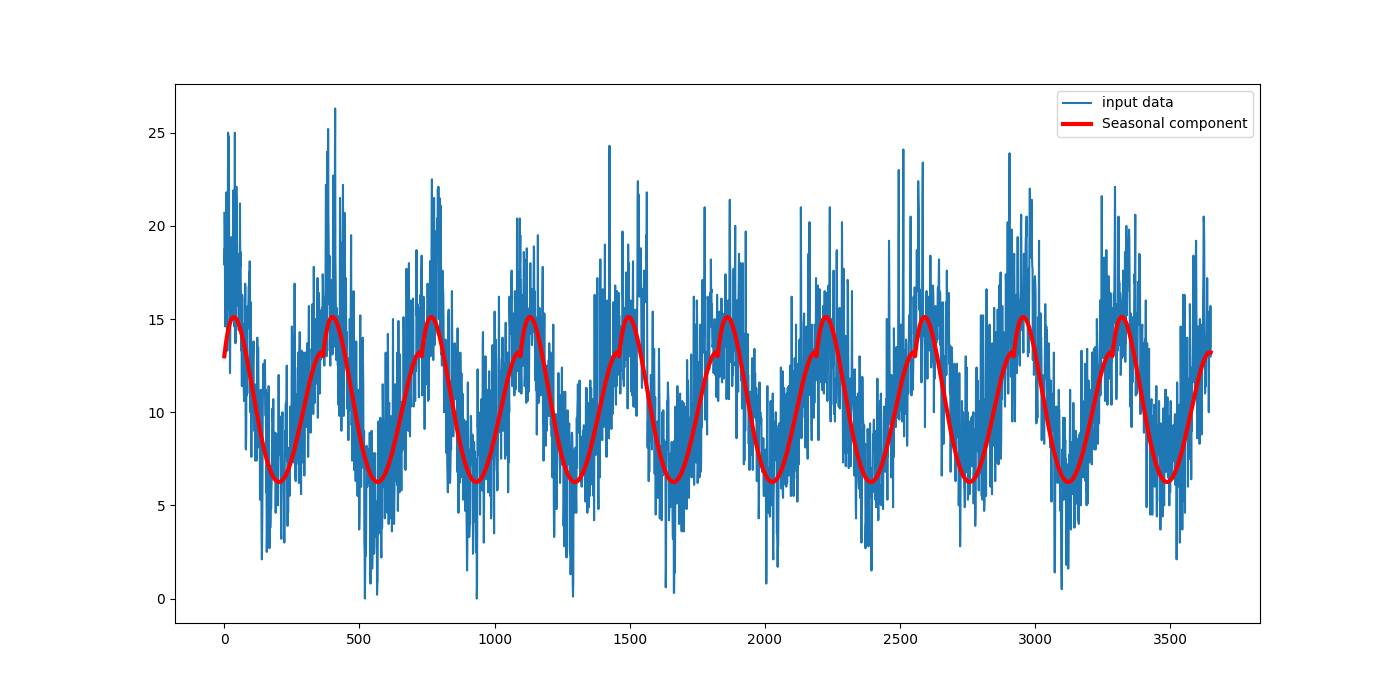
\includegraphics[width=\textwidth]{figures/Ass1/Ass1_D1_fiting_polynomial.png}
    \end{minipage}
    \caption{Seasonal component of the first dataset by fitting a polynomial (Degree of the polynomial is 4).}
    \label{fig:Ass1_D1_fiting_polynomial}
\end{figure}

\begin{figure}[H]
    \centering
    \begin{minipage}[b]{1\textwidth}
        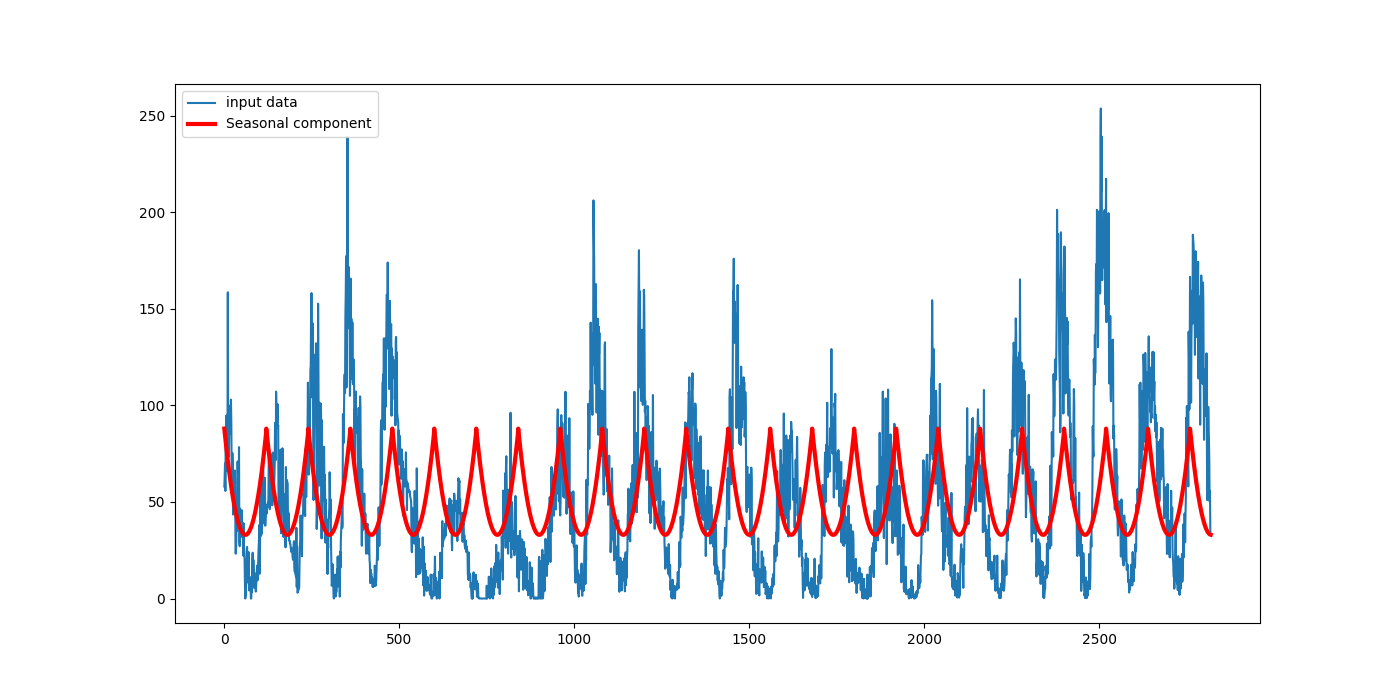
\includegraphics[width=\textwidth]{figures/Ass1/Ass1_D2_fiting_polynomial.png}
    \end{minipage}
    \caption{Seasonal component of the second dataset by fitting a polynomial (Degree of the polynomial is 2).}
    \label{fig:Ass1_D2_fiting_polynomial}
\end{figure}

\begin{figure}[H]
    \centering
    \begin{minipage}[b]{1\textwidth}
        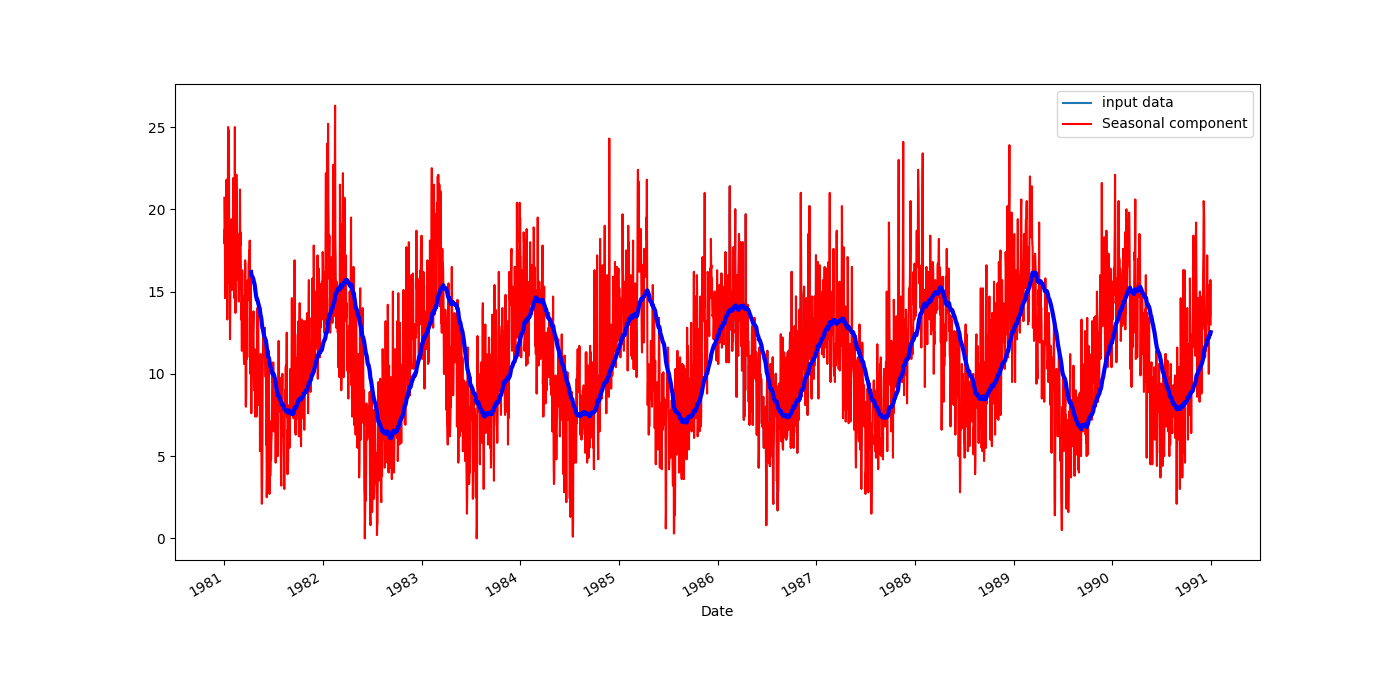
\includegraphics[width=\textwidth]{figures/Ass1/Ass1_D1_Moving_Avrage.png}
    \end{minipage}
    \caption{Seasonal component of the first dataset by Moving Average. The size of the window was set to 100.}
    \label{fig:Ass1_D1_Moving_Avrage}
\end{figure}

\begin{figure}[H]
    \centering
    \begin{minipage}[b]{1\textwidth}
        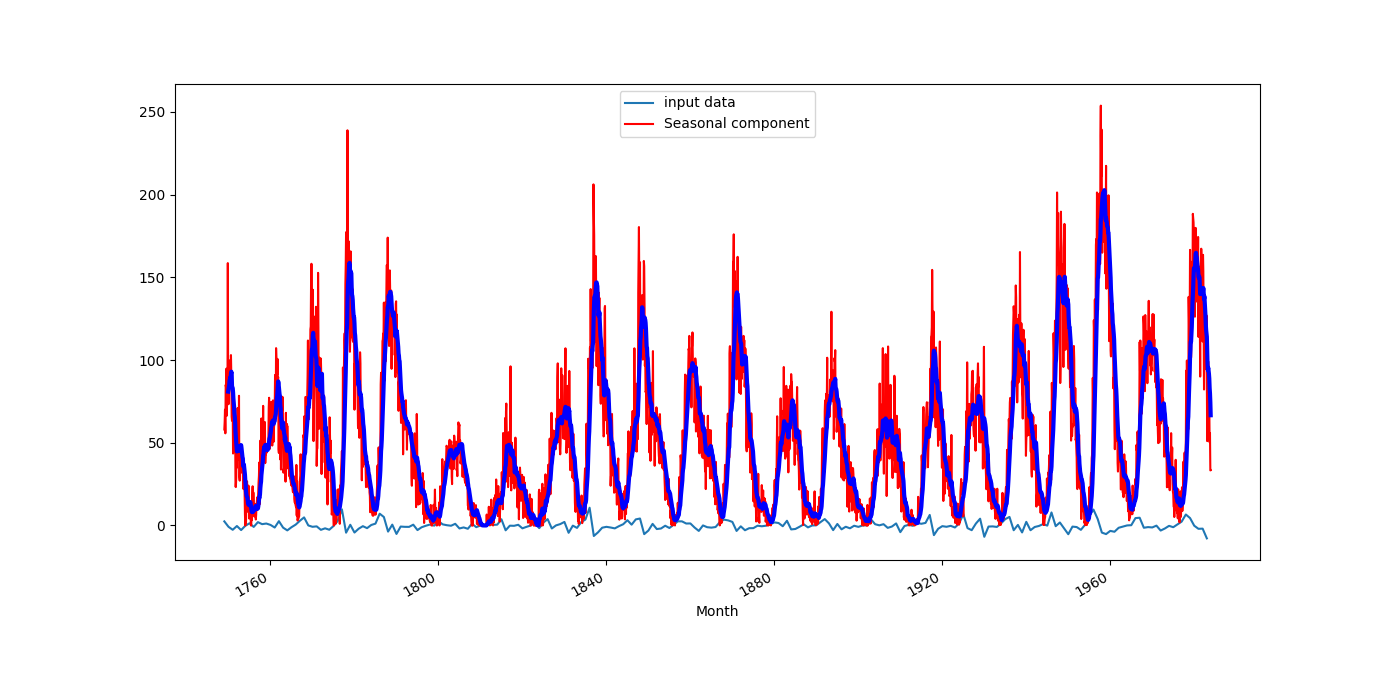
\includegraphics[width=\textwidth]{figures/Ass1/Ass1_D2_Moving_Avrage.png}
    \end{minipage}
    \caption{Seasonal component of the second dataset by Moving Average. The size of the window was set to 12.  }
    \label{fig:Ass1_D2_Moving_Avrage}
\end{figure}







%%%%%%%%%%%%%%%%%%%%%%%%%%%%%%%%%%%%%%%%%%%%%%%%%%%%%%%%%%%%%%%%%
%%%%%%%%%%%%%%%%%%%%%%%% Question 2 %%%%%%%%%%%%%%%%%%%%%%%%%%%%%
%%%%%%%%%%%%%%%%%%%%%%%%%%%%%%%%%%%%%%%%%%%%%%%%%%%%%%%%%%%%%%%%%
\item \textbf{For each dataset, examine the stationarity of the residuals using the ACF and PACF functions, Lag Plots, and/or other approaches. Show your results and provide commentary about your observations.}

\textit{\gls{ADF} shows that the time series is non-stationary or stationary. If the p-value is less than the significance level of 0.05 and the \gls{ADF} statistic is lower than one of the critical values, then the time series is stationary. For example, tables \ref{tab:Ass1_D1_ADF} and \ref{tab:Ass1_D2_ADF} shows the result of \gls{ADF} on a residual component of STL method in the two datasets.}

\begin{table}[H]
\centering
\caption{The result of the \gls{ADF} on the first dataset.}
\label{tab:Ass1_D1_ADF}
\begin{tabular}{lr}
\toprule
{} &            0 \\
\midrule
ADF Statistic               &   -24.697687 \\
p-value                     &     0.000000 \\
\#Lags Used                  &     3.000000 \\
Number of Observations Used &  3646.000000 \\
Critical Value (1\%)         &    -3.432145 \\
Critical Value (5\%)         &    -2.862333 \\
Critical Value (10\%)        &    -2.567192 \\
\bottomrule
\end{tabular}

\end{table}

\begin{table}[H]
\centering
\caption{The result of the \gls{ADF} on the second dataset.}
\label{tab:Ass1_D2_ADF}
\begin{tabular}{lr}
\toprule
{} &             0 \\
\midrule
ADF Statistic               & -1.128610e+01 \\
p-value                     &  1.416821e-20 \\
\#Lags Used                  &  2.700000e+01 \\
Number of Observations Used &  2.792000e+03 \\
Critical Value (1\%)         & -3.432694e+00 \\
Critical Value (5\%)         & -2.862576e+00 \\
Critical Value (10\%)        & -2.567321e+00 \\
\bottomrule
\end{tabular}

\end{table}



\textit{\gls{KPSS} is another test for checking the stationarity of a time series. If the p-value is less than the significance level of 0.05, then the time series is not stationary. Table \ref{tab:Ass1_D1_KPSS} and \ref{tab:Ass1_D2_KPSS} show the result of this test on STL residual.}

\begin{table}[H]
\centering
\caption{The result of the \gls{KPSS} on the first dataset.}
\label{tab:Ass1_D1_KPSS}
\begin{tabular}{lr}
\toprule
{} &          0 \\
\midrule
KPSS Statistic        &   0.318117 \\
p-value               &   0.100000 \\
Lags Used             &  22.000000 \\
Critical Value (10\%)  &   0.347000 \\
Critical Value (5\%)   &   0.463000 \\
Critical Value (2.5\%) &   0.574000 \\
Critical Value (1\%)   &   0.739000 \\
\bottomrule
\end{tabular}

\end{table}

\begin{table}[H]
\centering
\caption{The result of the \gls{KPSS} on the second dataset.}
\label{tab:Ass1_D2_KPSS}
\begin{tabular}{lr}
\toprule
{} &          0 \\
\midrule
KPSS Statistic        &   0.017052 \\
p-value               &   0.100000 \\
Lags Used             &  68.000000 \\
Critical Value (10\%)  &   0.347000 \\
Critical Value (5\%)   &   0.463000 \\
Critical Value (2.5\%) &   0.574000 \\
Critical Value (1\%)   &   0.739000 \\
\bottomrule
\end{tabular}

\end{table}

\textit{We can conclude that the series is stationary or not based on both \gls{KPSS} and \gls{ADF} \cite{StationarityStatsmodels}. Table \ref{tab:1} shows the possible outcomes of applying these two tests.}

\begin{table}[H]
\centering
\caption{The combination of the result of the \gls{KPSS} and \gls{ADF}.}
\label{tab:1}
% Please add the following required packages to your document preamble:
% \usepackage[table,xcdraw]{xcolor}
% If you use beamer only pass "xcolor=table" option, i.e. \documentclass[xcolor=table]{beamer}
\centering
\begin{tabular}{|l|l|l|}
\hline
KPSS test      & KDF test       & The combination result                      \\ \hline
non-stationary & non-stationary & The series is non-stationary.               \\ \hline
stationary     & non-stationary & Use detrending to make series stationary.   \\ \hline
non-stationary & stationary     & Use differencing to make series stationary. \\ \hline
stationary     & stationary     & The series is stationary.                   \\ \hline
\end{tabular}

\end{table}



\textit{\gls{ACF}  and \gls{PACF} plots allow you to determine the time series at zero hoe much correlation has with other lags. Figure \ref{fig:Ass1_D1_PACF_ACF} and \ref{fig:Ass1_D2_PACF_ACF} indicate these two plot for our datasets.}



\begin{figure}[H]
    \centering
    \begin{minipage}[b]{1\textwidth}
        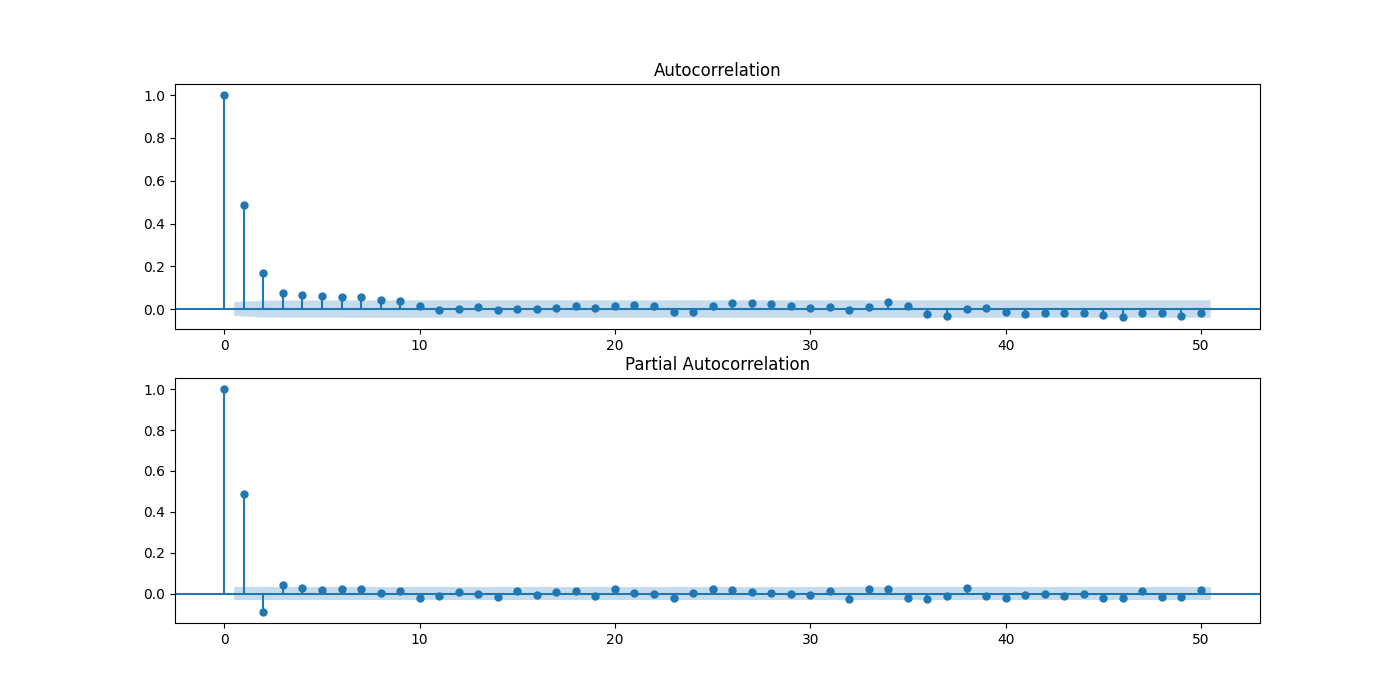
\includegraphics[width=\textwidth]{figures/Ass1/Ass1_D1_PACF_ACF.png}
    \end{minipage}
    \caption{A plot of the \gls{ACF} and \gls{PACF} of the first dataset.}
    \label{fig:Ass1_D1_PACF_ACF}
\end{figure}

\begin{figure}[H]
    \centering
    \begin{minipage}[b]{1\textwidth}
        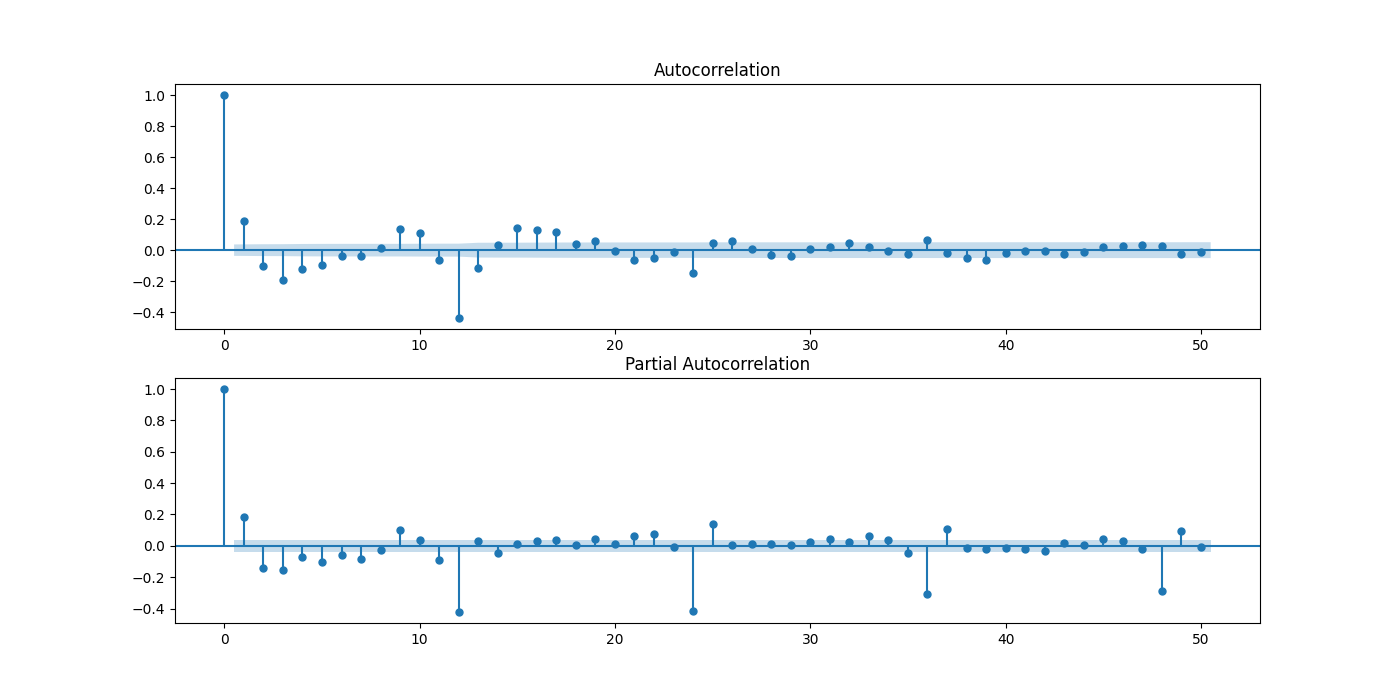
\includegraphics[width=\textwidth]{figures/Ass1/Ass1_D2_PACF_ACF.png}
    \end{minipage}
    \caption{A plot of the \gls{ACF} and \gls{PACF} of the second dataset.}
    \label{fig:Ass1_D2_PACF_ACF}
\end{figure}


\textit{These two plots are used to find the q and p for the ARIMA model. For example, if \gls{ACF} decays towards zero, and \gls{PACF} have only q significant value then our time series is a AR(q) process.}

\begin{table}[H]
\centering
\caption{The combination of the result of the \gls{KPSS} and \gls{ADF}.}
\label{tab:1}
% Please add the following required packages to your document preamble:
% \usepackage[table,xcdraw]{xcolor}
% If you use beamer only pass "xcolor=table" option, i.e. \documentclass[xcolor=table]{beamer}
\centering
\begin{tabular}{|l|l|l|}
\hline
KPSS test      & KDF test       & The combination result                      \\ \hline
non-stationary & non-stationary & The series is non-stationary.               \\ \hline
stationary     & non-stationary & Use detrending to make series stationary.   \\ \hline
non-stationary & stationary     & Use differencing to make series stationary. \\ \hline
stationary     & stationary     & The series is stationary.                   \\ \hline
\end{tabular}

\end{table}

\textit{The below figures (figure \ref{fig:Ass1_D1_Lag_Plots} and \ref{fig:Ass1_D2_Lag_Plots} ) show the lag plot of the two datasets. In each figure, there are four lag plots. As these plots illustrate, both datasets are linear, therefore our time series are a AR process.  }


\begin{figure}[H]
    \centering
    \begin{minipage}[b]{1\textwidth}
        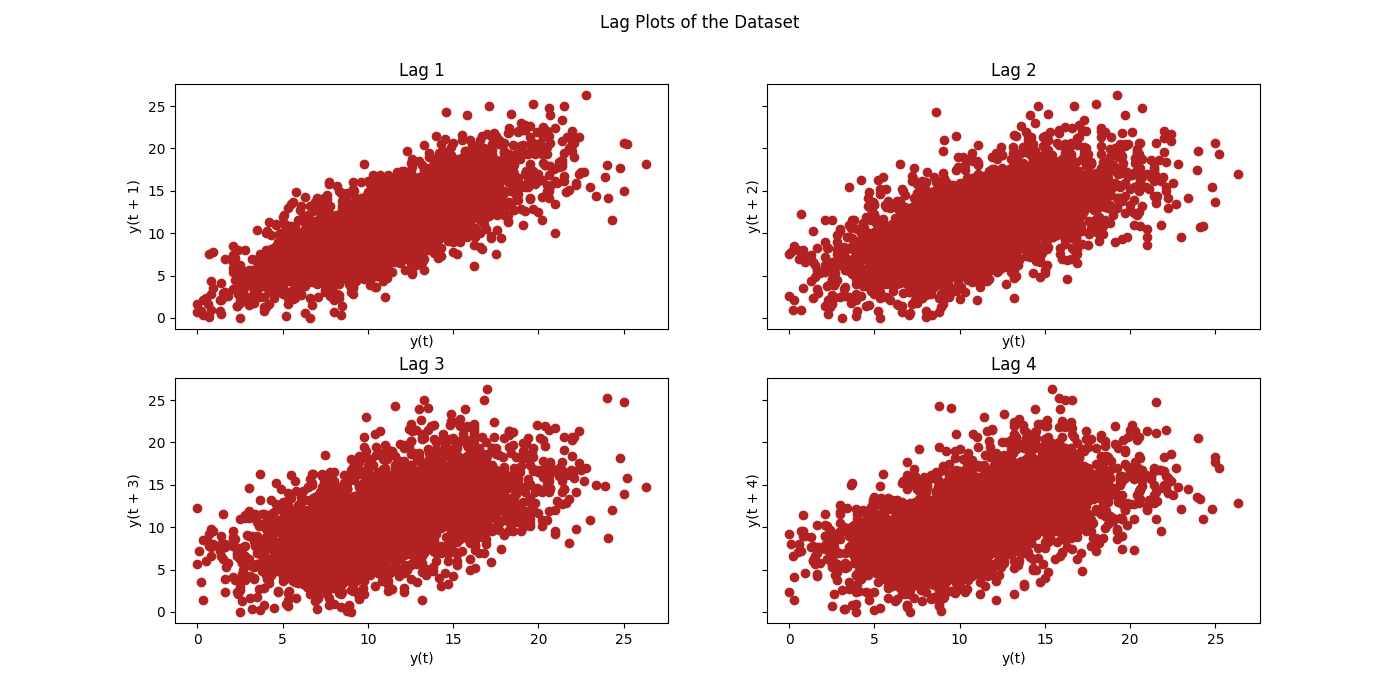
\includegraphics[width=\textwidth]{figures/Ass1/Ass1_D1_Lag_Plots.png}
    \end{minipage}
    \caption{A different lag plot of the first dataset.}
    \label{fig:Ass1_D1_Lag_Plots}
\end{figure}

\begin{figure}[H]
    \centering
    \begin{minipage}[b]{1\textwidth}
        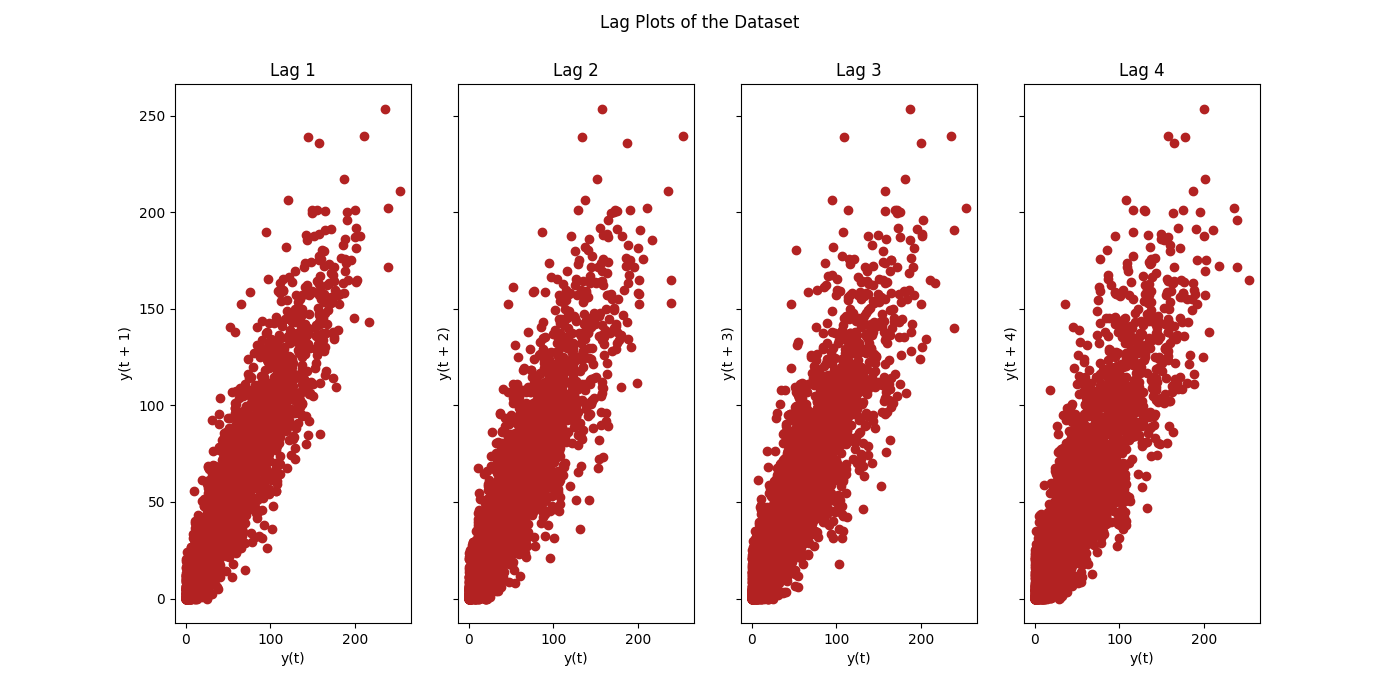
\includegraphics[width=\textwidth]{figures/Ass1/Ass1_D2_Lag_Plots.png}
    \end{minipage}
    \caption{A different lag plot of the second dataset.}
    \label{fig:Ass1_D2_Lag_Plots}
\end{figure}




\begin{figure}[H]
    \centering
    \begin{minipage}[b]{1\textwidth}
        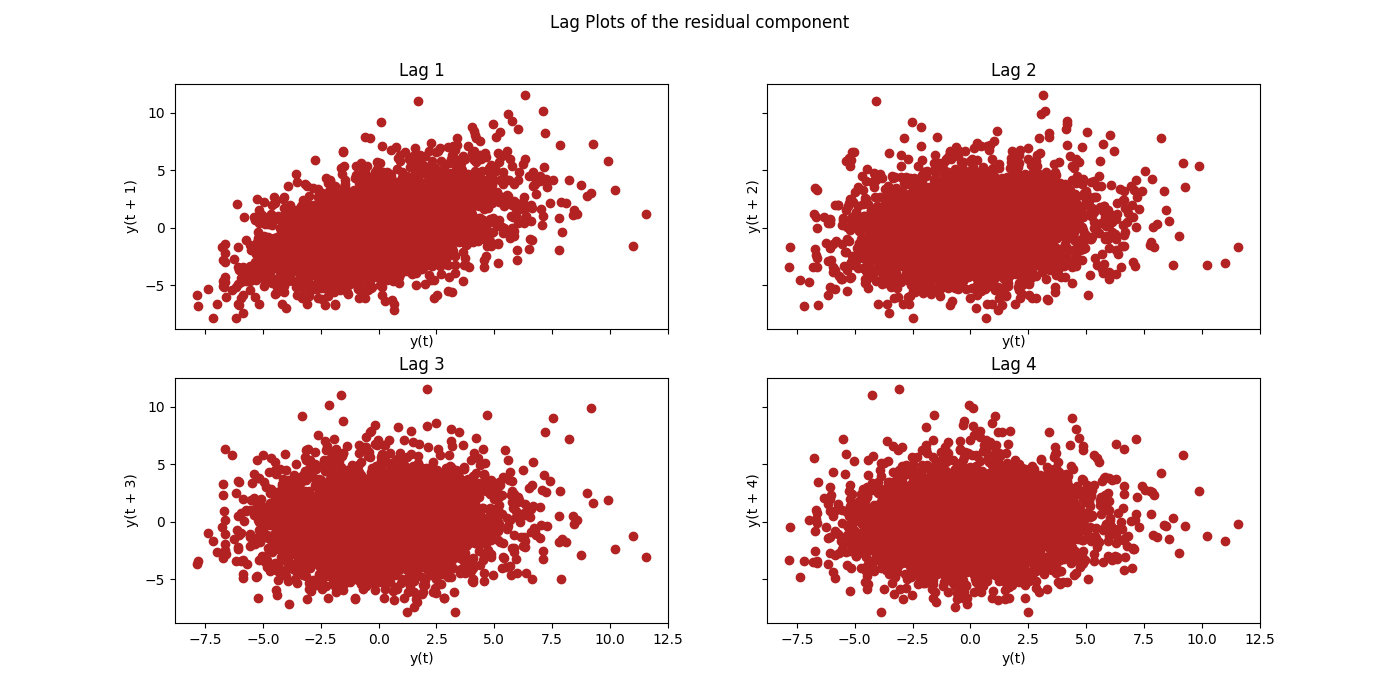
\includegraphics[width=\textwidth]{figures/Ass1/Ass1_D1_Lag_Plots_residual.png}
    \end{minipage}
    \caption{A different lag plot of residual component of the first dataset.}
    \label{fig:Ass1_D1_Lag_Plots_residual}
\end{figure}

\begin{figure}[H]
    \centering
    \begin{minipage}[b]{1\textwidth}
        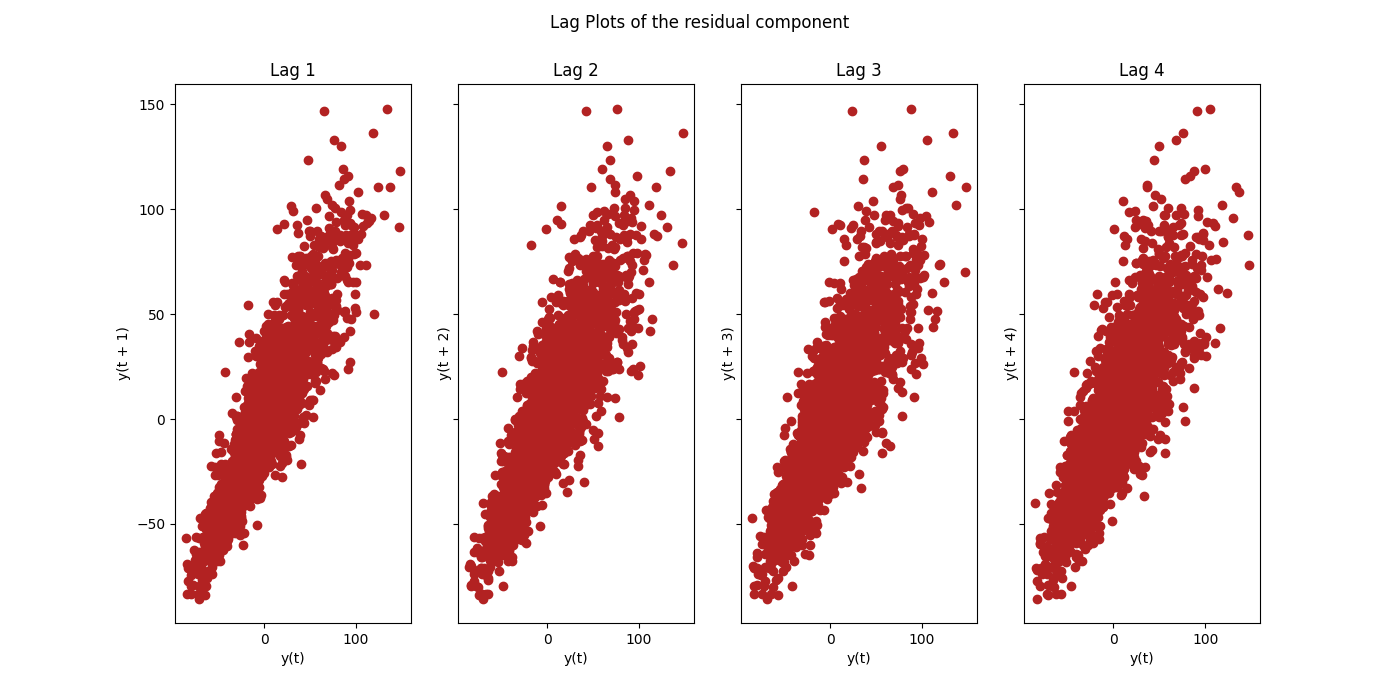
\includegraphics[width=\textwidth]{figures/Ass1/Ass1_D2_Lag_Plots_residual.png}
    \end{minipage}
    \caption{A different lag plot of residual component of the second dataset.}
    \label{fig:Ass1_D2_Lag_Plots_residual}
\end{figure}










%%%%%%%%%%%%%%%%%%%%%%%%%%%%%%%%%%%%%%%%%%%%%%%%%%%%%%%%%%%%%%%%%
%%%%%%%%%%%%%%%%%%%%%%%% Question 3 %%%%%%%%%%%%%%%%%%%%%%%%%%%%%
%%%%%%%%%%%%%%%%%%%%%%%%%%%%%%%%%%%%%%%%%%%%%%%%%%%%%%%%%%%%%%%%%
\item \textbf{Try modeling the residuals as an AR process. Use the tools at your disposal to decide on an appropriate order and analyse the results. What is the impact of selecting different orders on the remaining residuals?}

\textit{For this question, we need to select the order of the \gls{AR} term (p). Therefore, \gls{PACF} and \gls{ACF} were plotted at first (see figure \ref{fig:Ass1_D1_PACF_ACF_X}).}  

\begin{figure}[H]
    \centering
    \begin{minipage}[b]{1\textwidth}
        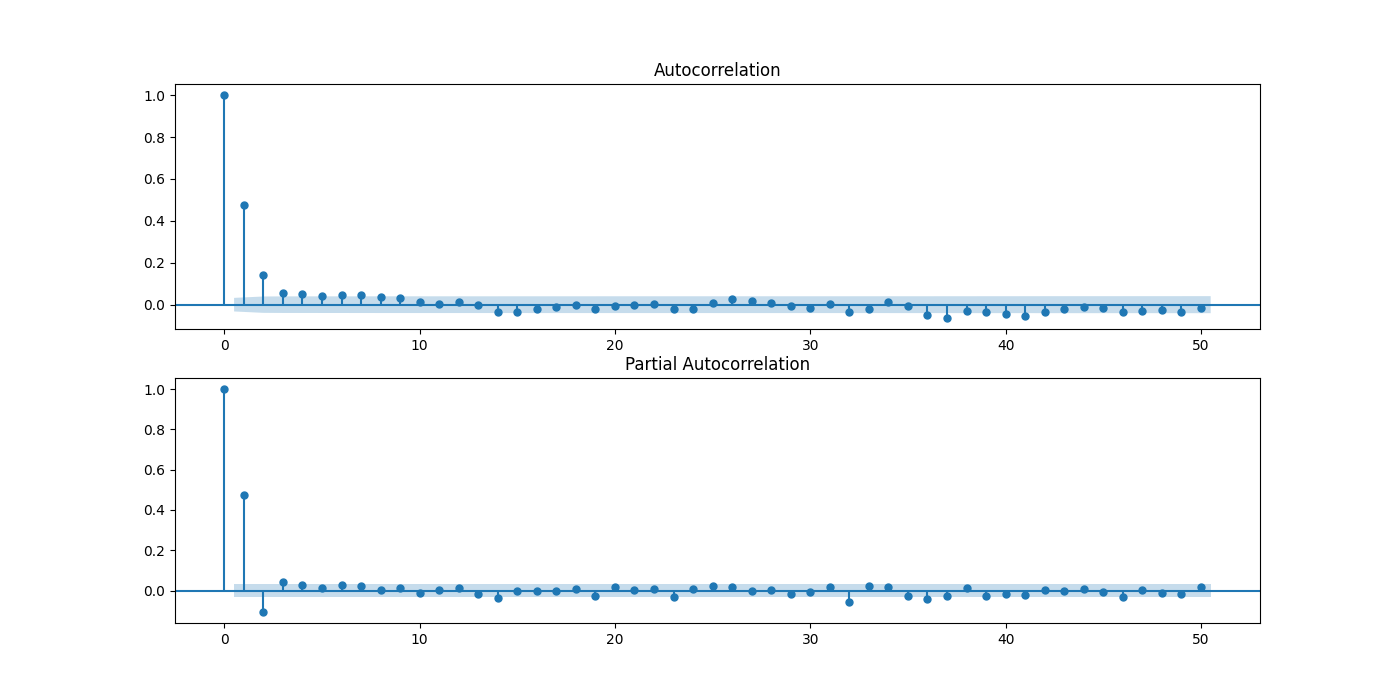
\includegraphics[width=\textwidth]{figures/Ass1/Ass1_D1_PACF_ACF_X.png}
    \end{minipage}
    \caption{A plot of the \gls{PACF} and \gls{ACF} of the residual part of the first dataset (residual of the STL method).}
    \label{fig:Ass1_D1_PACF_ACF_X}
\end{figure}

\textit{Sinse \gls{ACF} decaying (as figure \ref{fig:Ass1_D1_PACF_ACF_X} indicates), it can be concluded that the process is Auto Regressive. Also, based on PACF, the parameter of the \gls{AR} model should be start with an Auto Regressive model with lags 1 and 2 due to these two lags have a significant value.}



based on PACF we should start with an AR model with lags lags 1 ,2 ,10 ,13

so these are my starting points
must be stationary
these two plot do not tell us much


The PACF shows a single spike at the first lag and the ACF shows a tapering pattern. An AR(1) model is indicated.

2.How to find the order of the AR term (p)
\# PACF plot of 1st differenced series


You see how ACF is declining in amplitude exponentially, while PACF cuts off after lag 1. This may suggest that you\'re dealing with AR(1) process.

Note that the ACF shows exponential decay. This is indicative of a stationary series.

Note that the ACF shows an oscillation, indicative of a seasonal series. Note the peaks occur at lags of 12 months, 

The Akaike Information Critera (AIC) is a widely used measure of a statistical model. It basically quantifies 1) the goodness of fit, and 2) the simplicity/parsimony, of the model into a single statistic. When comparing two models, the one with the lower AIC is generally “better”.




%%%%%%%%%%%%%%%%%%%%%%%%%%%%%%%%%%%%%%%%%%%%%%%%%%%%%%%%%%%%%%%%%
%%%%%%%%%%%%%%%%%%%%%%%% Question 4 %%%%%%%%%%%%%%%%%%%%%%%%%%%%%
%%%%%%%%%%%%%%%%%%%%%%%%%%%%%%%%%%%%%%%%%%%%%%%%%%%%%%%%%%%%%%%%%
\item \textbf{Summarize your findings and observations briefly in a final discussion. Submit both the developed code and your document to the Assignment 1 folder on D2L.}

\textit{All files were uploaded on my GitHub repository \cite{}. The below table, shows the important paths of the project. Beside the codes are available in Appendix }

\begin{table}[H]
\centering
\begin{tabular}{|l|l|}
\hline
\multicolumn{2}{|l|}{The Important Paths:        } \\ \hline
\ \ \ \    ./EE6563/Dataset/Ass1             & Assignment datasets\\ \hline
\ \ \ \    ./EE6563/code/Ass1/sun.py         & Assignment code\\ \hline
\ \ \ \    ./EE6563/code/Ass1/Temp.py        & Assignment code\\ \hline
\ \ \ \    ./EE6563/manuscript/src/figures   & Assignment figures\\ \hline
\ \ \ \    ./EE6563/manuscript/src/tables    & Assignment table\\ \hline
\ \ \ \    ./EE6563/manuscript/src/Ass1.tex  & Assignment document\\ \hline
\end{tabular}
\end{table}











\end{enumerate}



\newpage
\bibliography{references}


\newpage
\section{Appendix (codes)}
\subsection{The script of Lab-1}

\begin{lstlisting}
%% Lab 1: Discrete-Time Frequency
% 
% Author: Maryhelen Stevenson
%
%% Explanation of the function ct_dt(.)
%
% The file ct_dt.m was supplied for use in this lab; a listing of the file
% is included in Appendix 1. The file defines a matlab function
% ct_dt(A,f0,PHI,fs,nc,ifig) which can be used to plot nc cycles
% of a continuous-time cosine with amplitude A, frequency f0, and phase
% PHI.  It also superimposes the values of the discrete-time sinusoid that
% would result from sampling the continuous-time sinusoid at a rate of fs
% samples per second.  The function returns a vector of time
% instances at which the values of the continuous-time sinusoid were
% evaluated to generate the continuous-time plot.
% 
% 
% An example to illustrate the usage of ct_dt(.) follows: 
%
close all
A = 2; % amplitude of continuous-time cosine
f0 = 0.5; % frequency (in units of Hz.) of continuous-time cosine
PHI = -pi/4; % phase (in units of radians) of continuous-time cosine
fs = 10; % sampling rate to be used (units of samples/second)
nc = 5; % number of cycles of continuous-time cosine to be plotted
ifig = 1; % optional figure number to use in the title of the figure
% the function returns the time vector used to plot the c.t. signal
t = ct_dt(A,f0,PHI,fs,nc,ifig); 

%%
% _Discussion of Figure 1_
% In accordance with the usage of ct_dt, we note that Figure 1,
% contains 5 cycles of the continuous-time cosine, $$x_a(t)$,
% where $$x_a(t)=2\cos(2\pi(0.5)t - \pi/4)$.  It also superimposes the 
% discrete-time sinusoid x[n] = xa(n/10).  The values of n are not shown
% but could be added in by hand.  Note that t=0 corresponds to n=0; whereas
% t=1 corresponds to n=10.
% etc.
% 
%% Exercise 1
%  
% Let x_a(t) = 3 sin(2 pi 50 t) = 3 cos (2 pi 50 t - pi/2)
% 
% Define x[n] = x_a(n/fs)
%
% a) Figure 2 shows a plot of xa(t) and x[n] for the case when fs=200
% samples/second.  It was produced using the code below.
% 
%  include the necessary code
close all
A = 3; 
f0 = 50; 
PHI = -pi/2; 
fs = 200; 
nc = 6;
ifig = 2; 


t = ct_dt(A,f0,PHI,fs,nc,ifig); 


%%
% _Discussion of Figure 2_
%
% include discussion here.  Your discussion should include answers to all
% questions posed in the lab manual.  Please use complete sentences.  Keep
% in mind that a reader should not have to have a copy of the lab manual to
% make sense of your discussion.
%%
% b) Figure 3 shows a plot of xa(t) and x[n] for the case when fs=120
% samples/second. It was produced using the code below.
% 
%  include the necessary code
fs = 120; 
ifig = 3; 


t = ct_dt(A,f0,PHI,fs,nc,ifig); 
%%
% _Discussion of Figure 3_
%
% include discussion here
%%
% c) Figure 4 shows a plot of xa(t) and x[n] for the case when fs=40
% samples/second. It was produced using the code below.
% 
%  include the necessary code 
fs = 40; 
ifig = 4; 


t = ct_dt(A,f0,PHI,fs,nc,ifig);
%%
% _Discussion of Figure 4_
%
% include discussion here.  
%
%%
% d) ...
%
%% Exercise 2
%
% 

close all
A = 6; 
f0 = 50; 
PHI = -pi/3; 
fs = 100; 
nc = 2;
ifig = 21; 


t = ct_dt(A,f0,PHI,fs,nc,ifig); 


A = 3; 
f0 = 50; 
PHI = 0; 
fs = 100; 
nc = 2;
ifig = 22; 


t = ct_dt(A,f0,PHI,fs,nc,ifig);


A = 6; 
f0 = 50; 
PHI = -pi/3; 
fs = 100; 
nc = 2;
ifig = 23; 


t = ct_dt(A,f0,PHI,fs,nc,ifig); 
y = 3*cos(2*pi*50*t);
plot(t,y,'*')
legend('x(t)','x[n]','y(t)')
%% Exercise 3
%
% 



close all
A = 1; 
f0 = 50; 
PHI = -pi/2; 
fs = 80; 
nc = 5;
ifig = 31; 


t = ct_dt(A,f0,PHI,fs,nc,ifig); 


y = cos(2*pi*30*t + pi/2);

plot(t,y,'*')
legend('x(t)','x[n]','y(t)')


%% Exercise 4
%
%
close all
A = 1; 
f0 = 60; 
PHI = 0; 
fs = 50; 
nc = 12;
ifig = 41; 


t = ct_dt(A,f0,PHI,fs,nc,ifig); 

y = cos(2*pi*10*t);

plot(t,y,'*')
legend('x(t)','x[n]','y(t)')

%% Appendix 1: Listing of the file ct_dt.m
%
%     Please include a listing of the function here, complete with any 
%     modifications that you may have made.
%
%     function t = ct_dt(A,f0,PHI,fs,nc, ifig)
%     %A 	    amplitude of cosine;
%     %f0 	CT frequency of cosine (cycles/sec);
%     %PHI 	phase of cosine (radians);
%     %fs	    sampling frequency (samples/sec.)
%     %nc 	number of CT cycles to be displayed
%     %ifig   optional Figure number to use in the title of the plot
%
%     ...

\end{lstlisting}
\subsection{The function of ct\_dt}
\begin{lstlisting}
function t = ct_dt(A,f0,PHI,fs,nc, ifig)
%A 	    amplitude of cosine;
%f0 	CT frequency of cosine (cycles/sec);
%PHI 	phase of cosine (radians);
%fs	    sampling frequency (samples/sec.)
%nc 	number of CT cycles to be displayed
%ifig   option Figure number to use in the title of the plot
%t      time vector used to plot CT cosine
if (nargin < 5 | nargin > 6)
    error('in call to ct_dt: there should be 5 arguments')
end
if (A < 0 )
    error(['in call to ct_dt: Amplitude of cosine, A,' ...
        'should not be negative'])
end
if (fs<0)
    error(['in call to ct_dt: the sampling frequency,'...
           ' fs,should be positive'])
end
if (nc<0)
    error('in call to ct_dt: nc should be positive')
end
if (exist('ifig'))
    pFig = ['Fig. ', num2str(ifig),':  '];
else
    pFig = [''];
end
    

figure, clf      
Ts=1/fs; %time between samples
Tp=1/abs(f0);  %period of CT cosine (sec/cycle)
F0 = f0/fs; %DT frequency (cycles/sample)
%DT plot will display samples n=0 to n=nmax
nmax = nc/abs(F0); 
%CT plot will display t=0 to t=tmax
tmax = nmax * Ts; 
% define t vector for CT plots to:
%  have a length greater than or equal to 200
%  with every kth element corresponding to a sampling instant
k = ceil(200/nmax);
t=0:Ts/k:tmax; 
xa = A*cos(2*pi*f0*t + PHI);
plot(t,xa);
hold on
n=0:nmax;
nTs = n*Ts;
xn = A*cos(2*pi*F0*n + PHI);
stem(nTs,xn);

p0=['x_a(t)=A cos(2\pi f_0 t), '];
p1=[' A='];
p2=[', f0='];
p3=[', PHI='];
p4=[', fs='];
p5=[', nc='];
p6=[', User='];
name=getenv('USER'); % gets the users login id
title( [pFig p0 p1 num2str(A) p2 num2str(f0) p3 num2str(PHI) ...
         p4 num2str(fs) p5 num2str(nc) p6 name ] )
xlabel('t (seconds), n')

\end{lstlisting}

\end{document}